\documentclass[12pt,a4paper]{report}
\usepackage[hidelinks]{hyperref}
\usepackage{geometry}
\usepackage{fancyhdr}
\setlength{\headheight}{14.5pt}
\usepackage{graphicx}
\usepackage{xcolor}
\usepackage{array}
\usepackage{booktabs}
\usepackage{tocloft}
\usepackage{colortbl}
\usepackage{float}
\usepackage{caption}
\usepackage{longtable}
\usepackage{amssymb}

\geometry{margin=1in}
\graphicspath{{images/}}

% Define colors for marking scheme
\definecolor{darkblue}{HTML}{1f4788}
\definecolor{lightblue}{HTML}{e8f1f8}

% Header and footer
\pagestyle{fancy}
\fancyhf{}
\rhead{Software Engineering G6046}
\lhead{Group Coursework Report}
\cfoot{\thepage}

% Title Page
\title{Software Engineering G6046 \\ \Large Clue! Coursework Report}
\author{Group 15}
\date{May 1, 2026}

\begin{document}
\pagenumbering{gobble}
\maketitle

\tableofcontents

\newpage
\chapter*{Marking Scheme}
\addcontentsline{toc}{chapter}{Marking Scheme}

This document is structured to address all marking criteria for the Software Engineering G6046 group coursework. The table below outlines each requirement, the maximum marks available, and where evidence of meeting that requirement can be found within this report.

\vspace{1cm}

\begin{center}
\begin{tabular}{|p{3.2cm}|p{1.5cm}|p{5.8cm}|p{2.2cm}|}
\hline
\rowcolor{darkblue}
\textcolor{white}{\textbf{Element}} &
\textcolor{white}{\textbf{Marks}} &
\textcolor{white}{\textbf{Description}} &
\textcolor{white}{\textbf{Link}} \\
\hline

Planning Docs (out of 5) & 5 & Project plan, PERT/Gantt charts, risk analysis & \hyperref[chap:planning]{\color{blue}\underline{Chapter \ref*{chap:planning}}} \\
\hline

Planning --- Meeting Notes (out of 5) & 5 & Meeting records, action tracking, team decisions & \hyperref[sect:meeting]{\color{blue}\underline{Section \ref*{sect:meeting}}} \\
\hline

Process Documentation (out of 10) & 10 & Sprint documentation, user stories, Agile evidence & \hyperref[chap:process]{\color{blue}\underline{Chapter \ref*{chap:process}}} \\
\hline

Design Documentation --- High Level (out of 5) & 5 & System architecture, component roles, interactions & \hyperref[chap:design-high]{\color{blue}\underline{Chapter \ref*{chap:design-high}}} \\
\hline

Design Documentation --- Low Level (out of 5) & 5 & Class diagrams, OO principles, API design & \hyperref[chap:design-low]{\color{blue}\underline{Chapter \ref*{chap:design-low}}} \\
\hline

Software Documentation (out of 5) & 5 & Code comments, XML DocStrings, IntelliSense cross-refs & \hyperref[chap:software]{\color{blue}\underline{Chapter \ref*{chap:software}}} \\
\hline

Testing Documentation (out of 10) & 10 & Unit tests, system tests, requirements traceability, edge cases & \hyperref[chap:process]{\color{blue}\underline{Chapter \ref*{chap:process}}} \\
\hline

Code (out of 50) & 50 & Working game, AI player, GUI, customisation & Submitted codebase \\
\hline

Group Report (out of 5) & 5 & Achievements, issues, critical analysis, team organisation & \hyperref[chap:project-overview]{\color{blue}\underline{Chapter \ref*{chap:project-overview}}} \\
\hline

\rowcolor{lightblue}
\textbf{TOTAL} & \textbf{100} & \textbf{Team Mark Base} & --- \\
\hline

\end{tabular}
\end{center}

\vspace{1em}

\noindent\textbf{Known gaps against the highest marking bands.} The following limitations prevent a full claim on the top band for some elements and are acknowledged explicitly in the report:

\begin{itemize}
    \item \textbf{Testing (9--10 band):} Sprint~4 system tests (S4.1--S4.12) were not fully executed before submission --- the Actual Result and Pass/Fail columns remain incomplete (Section~\ref{sec:sprint4}). Edge-case tests were performed for board movement (Sprint~3) but are not formally catalogued as a dedicated edge-case suite. Unit tests are linked to classes but not formally cross-referenced back to individual design artefacts (class diagram entries or sequence diagrams).
    \item \textbf{Code (41--50 band):} The AI player uses BFS-directed navigation toward envelope-candidate rooms and knowledge-filtered suggestions, but full notebook-based card-elimination deduction was not implemented (D3, KI-3 in Section~\ref{sec:sprint4-known-issues}). The player-count selector in the menu is not fully wired to \texttt{SceneController} (KI-1), and player names are not user-configurable --- Watson Games specifically identified customisation as a selling point. The game does not feature animated character movement or formally verified cross-platform (Mac/PC) operation.
\end{itemize}

\newpage


\pagenumbering{arabic}
\chapter{Planning Documentation}
\label{chap:planning}

\section{Project Plan}
\label{sect:planning}

This section details the project timeline, task allocations and risk management strategies for the Cluedo/Clue! Desktop Game, developed in \texttt{\texttt{C\#}} / Unity.

\subsection{Initial Gantt Chart}
The initial project timeline and task assignments are visualised in the Gantt chart (Figure \ref{fig:gantt_chart}). This chart and the accompanying breakdown in Table \ref{tab:gantt_tasks} represent the final of the project schedule, serving as combination of every individual Gantt chart developed during each sprint.
\begin{figure}[H]
    \centering
    
\includegraphics[width=\textwidth]{gantt.png}
    \caption{Unity project timeline (19 Feb -- 30 Apr 2026)}
    \label{fig:gantt_chart}
\end{figure}

\begin{table}[H]
    \centering
    \small
    \begin{tabular}{|p{6.2cm}|l|c|c|c|}
        \hline
        \textbf{Task} & \textbf{Owner(s)} & \textbf{Start} & \textbf{End} & \textbf{Status} \\ \hline
        Initial planning, meetings \& role assignments & All & 26 Jan & 19 Feb & Done \\ \hline
        Class diagram \& \texttt{cards.json} schema & Edward, Ethan & 19 Feb & 05 Mar & Done \\ \hline
        \texttt{Card}, \texttt{Deck} data classes \& \texttt{SceneController} & Ben, Edward & 19 Feb & 05 Mar & Done \\ \hline
        Unity project setup \& GitHub push & Matt & 19 Feb & 07 Mar & Done \\ \hline
        Repo tooling: Git LFS, PR templates, merge settings & Ethan, Edward & 05 Mar & 07 Mar & Done \\ \hline
        \texttt{BoardScript} (25$\times$24 tile array) & Matt & 10 Mar & 17 Mar & Done \\ \hline
        \texttt{GameManagerScript} singleton \& \texttt{GameState} & Ewan & 05 Mar & 17 Mar & Done \\ \hline
        \texttt{DiceRollScript} (physics) \& \texttt{MenuController} & Ben, Edward & 05 Mar & 17 Mar & Done \\ \hline
        \texttt{Player}/\texttt{HumanPlayer}/\texttt{TokenMover} (movement)$^*$ & Joe, Ethan & 17 Mar & 15 Apr & Done \\ \hline
        \texttt{UiManager}, \texttt{NotepadGrid} \& private modal & Matt & 17 Mar & 11 Apr & Done \\ \hline
        \texttt{RoomRules} (secret passages) \& \texttt{PlayTurn} coroutine & Ben, Ewan & 17 Mar & 11 Apr & Done \\ \hline
        \texttt{CharacterData} ScriptableObject \& JSON integration & Edward & 17 Mar & 11 Apr & Done \\ \hline
        \texttt{MainLoop}, suggestion \& accusation resolution & Ewan, Edward, Ethan & 14 Apr & 26 Apr & Done \\ \hline
        \texttt{AiPlayer} (BFS navigation, knowledge-filtered suggestions) & Ben & 14 Apr & 24 Apr & Done \\ \hline
        \texttt{PlayerKnowledge} \& \texttt{DoSuggestionThenAccusation} & Joe, Edward & 14 Apr & 26 Apr & Done \\ \hline
        \texttt{GameOverScreen} \& final UI polish & Matt & 14 Apr & 28 Apr & Done \\ \hline
        System testing, integration \& bug fixes & All & 18 Apr & 28 Apr & Done \\ \hline
        Documentation, report \& submission prep & Joe, All & 26 Apr & 30 Apr & Done \\ \hline
    \end{tabular}
    \caption{Final Consolidated Project Tasks and Timeline ($^*$Easter break 20~Mar -- 14~Apr: no development)}
    \label{tab:gantt_tasks}
\end{table}

\subsection{Critical Path}

The critical path runs through:

\begin{quote}
\textbf{BoardScript $\rightarrow$ GameManager $\rightarrow$ Deck/Cards $\rightarrow$ TokenMovement $\rightarrow$ GameLoop $\rightarrow$ Suggestion/Accusation $\rightarrow$ Win condition}
\end{quote}

Each task in this chain blocks the next: a player can only be \textit{placed} once the board exists; can only \textit{take a turn} once GameManager exists; can only \textit{move} once Deck/Cards is set up (the deck is built during game initialisation); can only \textit{make a Suggestion} once they are physically in a room (which requires TokenMovement); and can only \textit{win} via an Accusation evaluated against the solution envelope.

HandManager / CardInteraction sits on a \textit{parallel} branch off Deck/Cards --- Ben was able to develop the player hand UI during the same window as TokenMovement, so it does not appear on the critical path itself.

\subsubsection*{The Actual Bottleneck: TokenMovement}
TokenMovement was both the \textbf{longest single task} in the plan (17 Mar -- 15 Apr, $\sim$4 weeks) and the \textbf{task with the highest downstream impact} --- Suggestion, GameLoop progression, and AI movement all block on it. It was the right task to mark as the highest-risk item, and in practice it did slip slightly past its planned end date (see Revised Plan below).

\subsubsection*{Easter Break Disruption}
No development was scheduled or executed during the Easter holiday window (20 March -- 14 April). Effectively the critical path was paused for $\sim$3.5 weeks, which compressed Sprint 3 work into the second half of April and forced parallel execution of TokenMovement, GameLoop, and Suggestion in the final 10 days.

\subsection{Revised Plan}

The execution deviated from the initial Gantt in seven notable ways. They are recorded here so that a reader can compare the plan against what actually happened and understand why the team's structure changed during the project.

\begin{itemize}
    \item \textbf{Easter break paused development for $\sim$3.5 weeks:} There were \textbf{zero commits between 20 March and 14 April} on any branch. All the work nominally scheduled across the second half of Sprint 3 was compressed into the period 15--24 April.
    \item \textbf{TokenMovement slipped past its planned end date:} The major movement-fix commits actually landed on \textbf{17 April} and \textbf{18 April}. Legal-move detection on the irregular Cluedo board required more edge-case handling than the plan accounted for.
    \item \textbf{Suggestion / Accusation became a team task:} Originally assigned to Ewan, the work was distributed across Edward (guessing logic), Ethan (looping mechanisms), and Ewan (GameStateScript and menus) under time pressure.
    \item \textbf{Suggestion / Accusation logic merged into existing managers:} In the delivered codebase, the logic lives inside \texttt{GameManagerScript.cs} and \texttt{UiManager.cs} rather than in standalone classes. Splitting the classes cleanly would have required a refactor the team did not have time for (reflected in Chapter~\ref{chap:design-low}).
    \item \textbf{AI player scoped down:} The AI uses BFS-directed movement toward envelope-candidate rooms and knowledge-filtered suggestions; full notebook-based deduction (eliminating cards systematically) was not implemented (documented in Section~\ref{sec:sprint4}).
    \item \textbf{Sprint 2 absorbed unplanned repo infrastructure work:} Significant effort went into Git LFS setup, \texttt{.gitignore} fixes, PR templates, and Unity merge settings. This was necessary to prevent merge conflicts in Unity scenes but consumed feature development time.
    \item \textbf{Matt's script commits arrived late:} Matt's earlier work was contributed via pair-programming or was scene/asset work in Unity (which does not surface as distinct script commits). His first direct script commits in the repository arrived on 22--23 April.
\end{itemize}

\subsection{Effort Allocation}

Table \ref{tab:effort} shows the approximate hours per team member per sprint, estimated from Gantt task ownership, sprint-document contributions, and commit history. This justifies the peer-assessment split in Section~\ref{sec:peer-assessment}.

\begin{table}[H]
\centering
\caption{Effort Allocation (Approximate Hours)}
\label{tab:effort}
\begin{tabular}{|l|r|r|r|r|r|}
\hline
\textbf{Team Member} & \textbf{Sprint 1} & \textbf{Sprint 2} & \textbf{Sprint 3} & \textbf{Sprint 4} & \textbf{Total} \\ \hline
Edward & 8 & 12 & 14 & 18 & \textbf{52} \\ \hline
Ewan & 7 & 12 & 12 & 18 & \textbf{49} \\ \hline
Ethan & 8 & 9 & 14 & 14 & \textbf{45} \\ \hline
Joe & 7 & 8 & 14 & 16 & \textbf{45} \\ \hline
Ben & 5 & 9 & 11 & 14 & \textbf{39} \\ \hline
Matt & 6 & 9 & 10 & 15 & \textbf{40} \\ \hline
\textbf{Sprint Total} & \textbf{41} & \textbf{59} & \textbf{75} & \textbf{95} & \textbf{270} \\ \hline
\end{tabular}
\end{table}

\textit{Average 45 hours per person over the 10-week project (4.5 h/week).}
\subsection{Risk Analysis}

\subsubsection*{Risk Register}

\begin{table}[H]
\centering
\caption{Risk Register}
\label{tab:risk_register}
% This line forces the table to fit the text width
\resizebox{\textwidth}{!}{%
\begin{tabular}{|c|>{\centering\arraybackslash}p{4cm}|c|c|c|>{\centering\arraybackslash}p{4.5cm}|c|}
\hline
\textbf{ID} & \textbf{Risk} & \textbf{Likelihood} & \textbf{Impact} & \textbf{Severity} & \textbf{Mitigation Strategy} & \textbf{Owner} \\ \hline
R1 & Unity version incompatibility & 4 & 3 & High & Agree on LTS version; test in Sprint 1 & Matt \\ \hline
R2 & Git merge conflicts on scenes & 4 & 4 & High & Use UnityYAMLMerge; single owner per scene & Edward \\ \hline
R3 & Team member unable to contribute & 2 & 4 & Medium & Shared codebase knowledge; pair-coding & All \\ \hline
R4 & Scope creep & 3 & 3 & Medium & Prioritise core game loop first & Joe \\ \hline
R5 & Inconsistent physics dice & 3 & 2 & Medium & Fallback: default to 1 if result = 0 & Ben \\ \hline
R6 & AI player too complex & 3 & 2 & Low & Use random decision-making first & Ben \\ \hline
R7 & Corrupted submission file & 2 & 5 & Medium & Test zip unpacking before submission & Joe \\ \hline
R8 & Incomplete game loop & 2 & 5 & High & Prioritise end-to-end playable loop & All \\ \hline
R9 & Knowledge gap: Most of the team lacks prior experience with Unity or \texttt{C\#} & 5 & 4 & High & Allocate time in Sprint 1 for tutorials; pair-program with the experienced member & All \\ \hline
\end{tabular}%
} % Closes the resizebox
\end{table}

\subsubsection*{Risk Monitoring and Lessons Learned}

The team reviewed the risk register at the start of each sprint planning meeting.

\begin{itemize}
    \item \textbf{Sprint 1:} R1 was pre-empted. The team agreed on a Unity LTS version, and Edward seeded the repository with a working scene validated end-to-end. R9 materialised as the team's knowledge gap in Unity and C\# became apparent early on. To mitigate this, time was explicitly allocated in Sprint 1 for tutorials, and members relied heavily on pair-programming with the experienced team member to get up to speed.
    \item \textbf{Sprint 2:} R2 materialised (Unity scene merge conflicts) and R1 partially materialised (incomplete \texttt{.gitignore}). Ethan configured Git LFS, and Edward established Unity Smart Merge settings, PR compile-checks, and \texttt{.gitattributes} for \texttt{.unity} and \texttt{.prefab} files. The issue did not recur.
    \item \textbf{Sprint 3:} R3 materialised (the Easter break effectively paused all development for $\sim$3.5 weeks). R4 partially materialised as TokenMovement was more complex than estimated. The team scoped down TokenMovement, cutting A* pathfinding in favour of legal-move detection (documented in Section~\ref{sec:sprint3}).
    \item \textbf{Sprint 4:} R8 materialised (GameLoop, Suggestion, and AI were unfinished). R4 materialised via deliberate descoping under pressure. R2 re-emerged during the final integration push. Edward executed a large consolidate merge on 18 April. R7 was mitigated by verifying the zip unpacking before the deadline.
\end{itemize}

\textbf{Risks that did not materialise:}
R5 (physics dice fallback never triggered an invalid roll) and R6 (AI implementation was less difficult than expected, see section 2.4).

Lessons for Risk Planning:
\begin{enumerate}
    \item \textbf{Easter / holiday windows must be costed into the plan from the start.} Treating R3 as ``individual illness'' understated the systemic impact of a predictable shutdown.
    \item \textbf{Tool chain risks (R1, R2) have a higher early-impact than they appear.} Sprint 2 lost $\sim$1 week of feature work to repository tooling.
    \item \textbf{Scope-reduction is a valid mitigation.} Cutting some final UI tweaks preserved the critical path at the cost of design purity.
    \item \textbf{Account for learning curves in technical projects.} Identifying the knowledge gap (R9) early allowed the team to adjust Sprint 1 expectations, but future projects should formally budget time for upskilling.
\end{enumerate}

\newpage

% ==================== MEETING NOTES ====================
\section{Team Meetings}
\label{sect:meeting}

This section contains the records of all team meetings for the Clue! Simulation (G6046) project (Team 15: Ben, Edward, Ethan, Ewan, Joe, Matt). It details attendees, dates, summaries, agreed actions, and how risks were monitored and mitigated through decision-making.

\subsection{How to Read This Section}

\begin{quote}
The marking criterion for \textit{Planning -- meeting notes} (band 5) requires:
\textit{``A full set of notes that demonstrate an organised team, reflecting on progress on the project plan, and monitoring of risk factors identified, with appropriate mitigation through decision-making.''}

Each meeting below follows the same structure:
\begin{itemize}
    \item \textbf{Date / Duration / Attendees} --- for traceability and peer-assessment support.
    \item \textbf{Summary} --- what was discussed.
    \item \textbf{Decisions Made} --- outputs of the meeting (architectural, process, or planning).
    \item \textbf{Actions Agreed} --- owner-tagged tasks, each with a \textit{Completed?} column so the reader can see whether the action was actually delivered (band 4 requirement).
\end{itemize}

Cross-references: planning decisions feed the previous Project Plan section.
\end{quote}

\vspace{0.5cm}
\hrule
\vspace{0.5cm}

\subsection{Meeting 1}
\textbf{Date:} 26/01/2026 \\
\textbf{Duration:} $\sim$1 hour \\
\textbf{Attendees:} Ben, Edward, Ethan, Ewan, Joe, Matt

\subsubsection*{Summary}
\begin{itemize}
    \item Project briefing reviewed --- Watson Games' Cluedo simulation, desktop Mac/PC, with AI player and customisability requirements.
    \item Agreed to take a fluid approach to team roles --- tasks assigned based on who is best suited.
    \item Agreed to plan before deciding on a programming language.
    \item Began breaking down the classes that would be involved: Board, Players, Dice, Cards (Player, Room, Weapon), Grid of Judgements.
    \item Clarified the rules of the game.
    \item Agreed to use a statically typed language; discussed whether GUI should be 3D or 2D.
\end{itemize}

\subsubsection*{Decisions Made}
\begin{itemize}
    \item \textbf{Language/Platform:} Unity and \texttt{C\#} agreed upon (everyone in the group has little to no experience and would like to learn something new).
    \item \textbf{Frontend lead:} Matt.
    \item \textbf{Architecture:} Backend outputs a game state to the frontend, from which the frontend produces graphics.
    \item \textbf{Player branch:} One person to own the entire Player hierarchy (human and AI) to avoid confusion over inheritance.
    \item \textbf{Next meeting:} Monday the 1st.
\end{itemize}

\subsubsection*{Actions Agreed}
\begin{table}[H]
\centering
\resizebox{\textwidth}{!}{%
\begin{tabular}{|p{8cm}|l|l|}
\hline
\textbf{Action} & \textbf{Owner} & \textbf{Completed?} \\ \hline
Research Unity after meeting & All & Yes \\ \hline
Set up an empty Unity project as a ``spike'' to confirm everyone can run it & Edward & Yes --- initial commit 28/01 \\ \hline
Prepare for next meeting & All & Yes \\ \hline
\end{tabular}%
}
\end{table}

\vspace{0.5cm}
\hrule
\vspace{0.5cm}

\subsection{Meeting 2}
\textbf{Date:} 02/02/2026 \\
\textbf{Duration:} $\sim$1 hour 30 minutes \\
\textbf{Attendees:} Ben, Edward, Ethan, Ewan, Joe, Matt

\subsubsection*{Summary}
\begin{itemize}
    \item Reviewed Edward's Unity spike from the previous week --- confirmed the project compiles and runs on every team member's machine.
    \item Used the mark scheme to create a minimum viable plan, mapping out a full design plan and way of working.
    \item Agreed that the Board will be the main object in Unity --- parent to the majority of game parts.
    \item Agreed to make a skeleton code design of the entire game using a class diagram.
    \item Agreed to set up all specific documentation that the mark scheme mentions as we go through it.
    \item Agreed that after each commit to Git, each person is responsible for documenting what they have done.
    \item Agreed to create a schematic format for each commit to follow.
    \item Identified initial risks: Unity version drift between machines (R1) and Unity scene merge conflicts (R2) --- mitigations to be put in place before any feature work begins.
\end{itemize}

\subsubsection*{Decisions Made}
\begin{itemize}
    \item \textbf{Documentation:} Each person documents their own commits; a commit schematic format to be agreed and followed.
    \item \textbf{Design approach:} Class diagram to serve as the skeleton for the whole game.
    \item \textbf{Architecture:} Board as the main/parent object in Unity.
    \item \textbf{Risk register:} to be drafted formally and reviewed at every sprint planning meeting.
\end{itemize}

\subsubsection*{Actions Agreed}
\begin{table}[H]
\centering
\resizebox{\textwidth}{!}{%
\begin{tabular}{|p{8cm}|l|l|}
\hline
\textbf{Action} & \textbf{Owner} & \textbf{Completed?} \\ \hline
Create skeleton class diagram & Edward & Yes --- see \texttt{Design} docs \\ \hline
Agree commit schematic format & All & Yes --- followed across PRs \\ \hline
Set up documentation structure (\texttt{report/} folder) & Joe & Yes --- commits 19/02 \\ \hline
Draft initial risk register & Joe / Edward & Yes --- Table~\ref{tab:risk_register} \\ \hline
Continue building out basic Unity project structure & Edward & Yes --- commits 01/02 \\ \hline
\end{tabular}%
}
\end{table}

\vspace{0.5cm}
\hrule
\vspace{0.5cm}

\subsection{Meeting 3}
\textbf{Date:} 19/02/2026 \\
\textbf{Duration:} 1 hour 45 minutes \\
\textbf{Attendees:} Ben, Edward, Ethan, Ewan, Joe \textit{(Matt absent)}

\subsubsection*{Summary}
\begin{itemize}
    \item Agreed to use a standard format template for every meeting going forward.
    \item Main discussion centred around class structure.
    \item Sprint role assignments were started and partially agreed.
    \item Important game logic realisations and discussions took place.
    \item Decided to use XML comments for code documentation.
    \item Agreed sprint plan working backwards from deadline.
\end{itemize}

\subsubsection*{Decisions Made}

\textbf{Code Documentation:} \texttt{C\#} XML doc comments agreed as the standard.

\textbf{Privacy model discussed:} Options considered: (A) pass-and-play single screen, (B) cards hidden/revealed on demand via private modal, (C) split screen. \textbf{Agreed: Option B} --- Matt to implement a private modal in \texttt{UiManager} so revealed cards are shown only to the suggesting player.

\textbf{Data-driven design:} Board layout, character names, weapon names loaded from JSON files using Unity's built-in JsonUtility.

\begin{table}[H]
\centering
\caption*{Role Assignments}
\resizebox{\textwidth}{!}{%
\begin{tabular}{|l|p{8cm}|l|}
\hline
\textbf{Area} & \textbf{Scope} & \textbf{Assigned To} \\ \hline
\textbf{Game Logic \& Rules} & GameManager, turn flow, suggestions, accusations, win conditions & Ewan \\ \hline
\textbf{Board \& Movement} & Board grid, rooms, doors, pathfinding, secret passages & Joe, Ethan \\ \hline
\textbf{Card System} & Cards, dealing, murder envelope & Ben \\ \hline
\textbf{UI / GUI} & Board rendering, player HUD, detective notepad, menus & Matt \\ \hline
\textbf{Data Handling} & Loading/saving from JSON, designed data structure & Edward \\ \hline
\textbf{Diagrams \& Plans} & Gantt chart (or similar), UML diagram & Joe \\ \hline
\textbf{AI Player Agent} & Random agent first, then improved strategy if time allows & Ben \\ \hline
\textbf{Testing \& Docs} & Test plans, unit tests, sprint docs, meeting notes, report & Everyone \\ \hline
\end{tabular}%
}
\end{table}

\begin{table}[H]
\centering
\caption*{Sprint Plan}
\resizebox{\textwidth}{!}{%
\begin{tabular}{|l|l|p{8cm}|}
\hline
\textbf{Sprint} & \textbf{Focus} & \textbf{Key Deliverables} \\ \hline
Sprint 1 & Core logic & Board representation, player movement, turn system, dice, cards \\ \hline
Sprint 2 & Core gameplay & Suggestions, accusations, UI card logic, detective notes, rooms \\ \hline
Sprint 3 & AI \& polish & Random AI player agent, GUI polish, JSON loading \\ \hline
Sprint 4 & Testing \& docs & System/unit testing, bug fixes, documentation, final integration \\ \hline
\end{tabular}%
}
\end{table}

\subsubsection*{Actions Agreed}
\begin{table}[H]
\centering
\resizebox{\textwidth}{!}{%
\begin{tabular}{|p{6cm}|l|l|l|}
\hline
\textbf{Action} & \textbf{Owner} & \textbf{Due} & \textbf{Completed?} \\ \hline
Set up Unity project in GitHub repo & Matt & Next meeting & Yes (07 Mar) \\ \hline
Create shared documentation folder & Joe & Next meeting & Yes (19/02) \\ \hline
Write up retrospective notes for 1 \& 2 & Joe & Next meeting & Yes (19/02) \\ \hline
Draft initial Gantt chart / project plan & Joe & Next meeting & Yes \\ \hline
Design board data file schema (JSON) & Edward & --- & Yes \\ \hline
Create initial class diagram & Edward, Ethan & --- & Yes \\ \hline
Begin Sprint 1 work on assigned area & All & --- & Yes \\ \hline
\end{tabular}%
}
\end{table}

\vspace{0.5cm}
\hrule
\vspace{0.5cm}

\subsection{Meeting 4}
\textbf{Date:} 05/03/2026 \\
\textbf{Duration:} $\sim$1 hour \\
\textbf{Attendees:} Ben, Edward, Ethan, Ewan, Joe, Matt

\subsubsection*{Summary}
\begin{itemize}
    \item \textbf{Sprint 1 close.} Reviewed deliverables: Deck and Card classes, JSON schema, basic Unity scene with placeholder board.
    \item Discussion on whether sprint roles need to change for Sprint 2. Agreed the \textit{Tiles and Board} role is no longer a separate area; absorbed into Matt's UI ownership.
    \item Reviewed risks. R1 (Unity version) had not materialised. R2 (merge conflicts) flagged as the next likely risk now that real feature work was about to begin in parallel.
    \item Agreed Sprint 2 priorities: BoardScript, GameManagerScript singleton, DiceRollScript with physics, token spawning, repo clean-up / Git LFS.
    \item Brief retrospective: documentation kept up; commit schematic being followed inconsistently --- agreed to enforce more strictly via the PR template.
\end{itemize}

\subsubsection*{Decisions Made}
\begin{itemize}
    \item \textbf{Role change:} Tiles and Board role removed as a separate area; responsibilities absorbed into UI (Matt).
    \item \textbf{Sprint 1 closed.} All Sprint 1 objectives met.
    \item \textbf{Sprint 2 plan:} Core gameplay infrastructure. Repo tooling (Git LFS, \texttt{.gitattributes}, PR templates) to be set up \textit{before} any feature work to mitigate R2.
    \item \textbf{PR-template enforcement:} Edward to add a ``large PR'' warning workflow and a Unity compile-check workflow on PRs.
\end{itemize}

\subsubsection*{Actions Agreed}
\begin{table}[H]
\centering
\resizebox{\textwidth}{!}{%
\begin{tabular}{|p{6cm}|l|l|l|}
\hline
\textbf{Action} & \textbf{Owner} & \textbf{Due} & \textbf{Completed?} \\ \hline
Set up Git LFS and clean up the repo & Ethan & Before Sp 2 & Yes (06/03) \\ \hline
Add PR templates, compile checks & Edward & Before Sp 2 & Yes (07/03) \\ \hline
Add Unity smart merge settings & Edward & Before Sp 2 & Yes (07/03) \\ \hline
Begin \texttt{BoardScript} (25$\times$24 tile encoding) & Matt & Sprint 2 & Yes (10/03) \\ \hline
Begin \texttt{GameManagerScript} (setup) & Ewan & Sprint 2 & Yes \\ \hline
Begin \texttt{DiceRollScript} (Rigidbody) & Ben & Sprint 2 & Yes \\ \hline
Refine class diagram alongside dev & Edward, Ethan & Ongoing & Yes \\ \hline
\end{tabular}%
}
\end{table}

\vspace{0.5cm}
\hrule
\vspace{0.5cm}

\subsection{Meeting 5}
\textbf{Date:} 10/03/2026 \\
\textbf{Duration:} $\sim$1 hour 30 minutes \\
\textbf{Attendees:} Ben, Edward, Ethan, Ewan, Joe, Matt

\subsubsection*{Summary}
\begin{itemize}
    \item Mid-Sprint-2 check-in. Repo tooling from Meeting 4 had landed --- confirmed merge conflicts no longer breaking the build.
    \item Detailed discussion on the division of backend work and Matt's frontend. Agreed \texttt{GameManagerScript} is the bridge; UI scripts should never read the board state directly.
    \item Matt walked the team through the Unity editor, scene hierarchy, and \texttt{MonoBehaviour} lifecycle methods. Important for backend-focused members.
    \item Edward flagged that the current \texttt{DeckScript} was blocking progress on \texttt{GameManagerScript}. Agreed Edward would lead a Deck refactor.
    \item Discussed turn-order --- agreed to hardcode standard Cluedo order for simplicity.
\end{itemize}

\subsubsection*{Decisions Made}
\begin{itemize}
    \item \textbf{Backend / frontend boundary:} \texttt{GameManagerScript} is the single bridge. Matt's UI consumes its API.
    \item \textbf{Customisation:} Character names, weapons, room names loaded from \texttt{cards.json}. Adding/changing a card requires only a JSON edit.
    \item \textbf{Deck refactor:} Edward to refactor \texttt{DeckScript} so it initialises cleanly from GameManager.
    \item \textbf{Turn order:} Hardcoded as Miss Scarlett $\rightarrow$ Mustard $\rightarrow$ White $\rightarrow$ Green $\rightarrow$ Peacock $\rightarrow$ Plum.
\end{itemize}

\subsubsection*{Actions Agreed}
\begin{table}[H]
\centering
\resizebox{\textwidth}{!}{%
\begin{tabular}{|p{8cm}|l|l|}
\hline
\textbf{Action} & \textbf{Owner} & \textbf{Completed?} \\ \hline
Refactor \texttt{DeckScript} so it initialises from GameManager & Edward & Yes (11/03) \\ \hline
Continue \texttt{GameManagerScript} (singleton + setup) & Ewan & Yes (17/03) \\ \hline
Begin token spawning logic in \texttt{GameManagerScript} & Edward & Yes (17/03) \\ \hline
Flesh out \texttt{PlayerScripts} (player state container) & Joe & Yes (17/03) \\ \hline
Finalise \texttt{Card} / \texttt{Deck} data classes & Ben & Yes (17/03) \\ \hline
Confirm \texttt{cards.json} covers 6 chars, 6 weapons, 9 rooms & Edward & Yes \\ \hline
\end{tabular}%
}
\end{table}

\vspace{0.5cm}
\hrule
\vspace{0.5cm}

\subsection{Meeting 6}
\textbf{Date:} 17/03/2026 \\
\textbf{Duration:} $\sim$1 hour \\
\textbf{Attendees:} Ben, Edward, Ethan, Ewan, Joe, Matt

\subsubsection*{Summary}
\begin{itemize}
    \item Sprint 2 review --- board, game manager, dice and token spawning working.
    \item Decision made to formalise a \texttt{GameState} singleton to manage Playing/MainMenu/GameOver instead of handling it ad hoc.
    \item Reviewed role assignments --- board/tiles work largely complete so Joe and Ethan to shift focus to \texttt{TokenMovementScript}.
    \item Discussed how to handle turn sequence --- Ewan to own the main loop.
    \item Edward to look into how \texttt{SceneController} persists data.
\end{itemize}

\subsubsection*{Decisions Made}
\begin{itemize}
    \item \textbf{GameState singleton} to manage game-wide state transitions.
    \item \textbf{SceneController} to use \texttt{DontDestroyOnLoad} to persist player counts.
    \item Board/tile work considered done; Joe and Ethan move to movement.
\end{itemize}

\subsubsection*{Actions Agreed}
\begin{table}[H]
\centering
\resizebox{\textwidth}{!}{%
\begin{tabular}{|p{8cm}|l|l|}
\hline
\textbf{Action} & \textbf{Owner} & \textbf{Completed?} \\ \hline
Implement \texttt{GameState} & Ewan & Yes \\ \hline
Begin \texttt{TokenMovementScript} & Joe, Ethan & Yes \\ \hline
Integrate \texttt{DiceRollScript} result into turn start & Ben & Yes \\ \hline
Finalise \texttt{SceneController} with DontDestroyOnLoad & Edward & Yes \\ \hline
Begin \texttt{MenuController} scene transition & Edward & Yes \\ \hline
\end{tabular}%
}
\end{table}

\vspace{0.5cm}
\hrule
\vspace{0.5cm}

\subsection{Meeting 7}
\textbf{Date:} 31/03/2026 \\
\textbf{Duration:} $\sim$1 hour 15 minutes \\
\textbf{Attendees:} Ben, Edward, Ethan, Ewan, Joe, Matt

\subsubsection*{Summary}
\begin{itemize}
    \item Sprint 3 progress review --- token movement working for basic corridor navigation.
    \item Identified issue: two competing implementations in \texttt{TokenMovementScript} (int array vs Vector2Int). Agreed to keep Vector2Int.
    \item Discussed card reveal during suggestions --- Matt to handle private modal.
    \item Room entry needs mapping door tile values (2--11) to strings.
    \item Discussed AI --- agreed random legal moves are sufficient.
\end{itemize}

\subsubsection*{Decisions Made}
\begin{itemize}
    \item \textbf{\texttt{Vector2Int}} adopted as standard; old \texttt{int[]} movement approach removed.
    \item \textbf{\texttt{UiManager}} to be the single point of contact for all player-facing UI.
    \item \textbf{Room mapping} to map door IDs 2--11 to room names.
    \item \textbf{AI movement:} random selection from \texttt{GetLegalMoves()} --- no A* pathfinding.
\end{itemize}

\subsubsection*{Actions Agreed}
\begin{table}[H]
\centering
\resizebox{\textwidth}{!}{%
\begin{tabular}{|p{8cm}|l|l|}
\hline
\textbf{Action} & \textbf{Owner} & \textbf{Completed?} \\ \hline
Clean up \texttt{TokenMovementScript} --- remove old \texttt{int[]} & Joe & Yes \\ \hline
Implement \texttt{TokenMover.EnterRoom()} \& string mapping & Ben & Yes \\ \hline
Complete \texttt{UiManager} prompts and private modal & Matt & Yes \\ \hline
Implement \texttt{NotepadGrid} toggle UI & Matt & Yes \\ \hline
Wire AI random move into \texttt{PlayTurn} coroutine & Ewan, Joe & Yes \\ \hline
Everyone write up own contribution notes & All & Partially (in Sp 4) \\ \hline
\end{tabular}%
}
\end{table}

\vspace{0.5cm}
\hrule
\vspace{0.5cm}

\subsection{Meeting 8}
\textbf{Date:} 14/04/2026 \\
\textbf{Duration:} $\sim$1 hour \\
\textbf{Attendees:} Ben, Edward, Ethan, Ewan, Joe \textit{(Matt absent)}

\subsubsection*{Summary}
\begin{itemize}
    \item Sprint 3 close --- prototype playable to the point of entering rooms.
    \item Ewan identified suggestion \textit{resolution} (clockwise card-showing) as the most complex remaining piece; top priority for Sprint 4.
    \item Noted \texttt{MenuController} hardcoded counts --- logged as known issue.
    \item Ben to complete AI suggestion generation.
    \item \texttt{GameOverScreen} needed for end state.
    \item Submission deadline reminder: 30 April, 4PM.
\end{itemize}

\subsubsection*{Decisions Made}
\begin{itemize}
    \item \textbf{Sprint 4 priority:} (1) Suggestion resolution, (2) Accusation, (3) AI suggestions, (4) Game over screen, (5) Docs.
    \item \textbf{Known issues logged:} Hardcoded menu counts and spawn issues with $<$ 6 players will be documented rather than delaying Sprint 4 logic.
\end{itemize}

\subsubsection*{Actions Agreed}
\begin{table}[H]
\centering
\resizebox{\textwidth}{!}{%
\begin{tabular}{|p{8cm}|l|l|}
\hline
\textbf{Action} & \textbf{Owner} & \textbf{Completed?} \\ \hline
Implement \texttt{ResolveSuggestion()} clockwise coroutine & Ewan & In progress \\ \hline
Implement accusation check vs \texttt{GetEnvelope()} & Ewan & In progress \\ \hline
AI random suggestion when in room & Ben & In progress \\ \hline
\texttt{GameOverScreen} --- restart and return-to-menu & Matt & Yes \\ \hline
Fill sprint docs and report skeleton & Joe, All & In progress \\ \hline
Record any known bugs for testing documentation & All & In progress \\ \hline
\end{tabular}%
}
\end{table}

\vspace{0.5cm}
\hrule
\vspace{0.5cm}

\subsection{Meeting 9}
\textbf{Date:} 20/04/2026 \\
\textbf{Duration:} $\sim$45 minutes \\
\textbf{Attendees:} Ben, Edward, Ethan, Ewan, Joe \textit{(Matt absent)}

\subsubsection*{Summary}
\begin{itemize}
    \item Sprint 4 mid-point check-in. Ewan demoed suggestion resolution working end-to-end.
    \item Accusation logic implemented. Incorrect accusation eliminates player.
    \item AI player takes full turns (rolls, moves, enters rooms, suggests).
    \item \texttt{GameOverScreen} wired up and working.
    \item Discussed peer assessment and final submission logistics.
\end{itemize}

\subsubsection*{Decisions Made}
\begin{itemize}
    \item Accusation to be offered as an option after a suggestion is resolved, not as a separate mandatory step.
    \item Known issues formally documented rather than attempting a last-minute fix.
    \item Final submission ZIP to be verified by group before uploading.
\end{itemize}

\subsubsection*{Actions Agreed}
\begin{table}[H]
\centering
\resizebox{\textwidth}{!}{%
\begin{tabular}{|p{8cm}|l|l|}
\hline
\textbf{Action} & \textbf{Owner} & \textbf{Completed?} \\ \hline
Wire accusation UI option after suggestion resolution & Ewan & In progress \\ \hline
Fix / document $<$ 6 player token spawn issue & Ethan & In progress \\ \hline
Fill all sprint doc test result columns & All & In progress \\ \hline
Complete group report (achievements, lessons) & Joe & In progress \\ \hline
Agree peer assessment marks & All & Before 30 Apr \\ \hline
Record gameplay video (MP4) & Matt & Before 29 Apr \\ \hline
Final submission ZIP upload to Canvas & TBC & By 30 Apr 4PM \\ \hline
\end{tabular}%
}
\end{table}

\newpage

\chapter{Process Documentation}
\label{chap:process}

\section{Agile Process Evidence}

The project followed four two-to-three week Agile sprints running from 19 February to 30 April 2026.
Each sprint produced a working increment and closed with a retrospective that fed directly into the next sprint plan.
The evidence for each sprint is structured as: summary data, individual contributions, user stories, requirements, design decisions, test results, and retrospective.

% ---- SPRINT 1 ----
\section{Sprint 1 --- Project Setup, Architecture \& Core Data}
\label{sec:sprint1}

\subsection*{Summary Data}
\begin{tabular}{ll}
\textbf{Team Number:} & 15 \\
\textbf{Sprint Technical Lead:} & Edward (Unity setup, class diagram, JSON schema) \\
\textbf{Start Date:} & 19 February 2026 \\
\textbf{End Date:} & 05 March 2026 \\
\end{tabular}

\subsection*{Individual Key Contributions}
\begin{table}[H]
\centering
\resizebox{\textwidth}{!}{%
\begin{tabular}{|l|p{10cm}|}
\hline
\textbf{Team Member} & \textbf{Key Contribution(s)} \\ \hline
Matt & Created initial Unity project (\texttt{clue}); pushed to GitHub; established project structure \\ \hline
Ewan & Game logic architecture; turn flow and class responsibility design \\ \hline
Joe & Board and movement design; initial board representation planning \\ \hline
Ethan & Board and movement design; room and corridor layout planning \\ \hline
Ben & Card system: \texttt{Card} class, \texttt{Deck} class, \texttt{CardType} enum \\ \hline
Edward & Data handling: designed \texttt{cards.json} external data file; \texttt{SceneController} \\ \hline
\end{tabular}%
}
\end{table}

\subsection*{User Stories}

\textbf{US1 -- Shared Development Environment:} As a development team, we need a shared, runnable Unity project on GitHub so that all team members can contribute from a common baseline. (Priority: Critical)

\textbf{US2 -- Card \& Deck Data Structures:} As a developer, I need card and deck data structures so that subsequent sprints can implement dealing, hand management and the murder envelope. (Priority: High)

\textbf{US3 -- Scene-to-Scene Data Passing:} As a developer, I need player and AI count to persist from the menu scene to the game scene so that the game can be configured before starting. (Priority: High)

\subsection*{Requirements Analysis}

\textbf{Functional Requirements (Mandatory):}
\begin{itemize}
    \item \textbf{F1.1} A shared version-controlled repository accessible to all team members.
    \item \textbf{F1.2} Unity (C\#) as the implementation platform.
    \item \textbf{F1.3} \texttt{Card} stores a \texttt{CardType} enum (Person / Weapon / Room), a name string, and an integer ID.
    \item \textbf{F1.4} \texttt{Deck} loads card names from \texttt{StreamingAssets/cards.json} via \texttt{JsonUtility}.
    \item \textbf{F1.5} Three cards (one of each type) are selected as the murder envelope before dealing.
    \item \textbf{F1.6} Remaining 18 cards are dealt to active players one at a time, round-robin.
    \item \textbf{F1.7} Player count and AI count persist from menu to game scene via \texttt{SceneController}.
\end{itemize}

\textbf{Functional Requirements (Desirable):}
\begin{itemize}
    \item \textbf{F1.8} Character, weapon, and room names configurable via \texttt{cards.json} without recompiling.
\end{itemize}

\textbf{Non-Functional Requirements:}
\begin{itemize}
    \item \textbf{NF1.1} Project compiles and runs on all team members' machines by sprint close.
    \item \textbf{NF1.2} C\# XML \texttt{///} doc comment format as the documentation standard.
\end{itemize}

\textbf{Domain Requirements:}
\begin{itemize}
    \item \textbf{D1.1} Exactly 6 persons, 6 weapons, and 9 rooms --- 21 cards total.
    \item \textbf{D1.2} One person, one weapon, one room card in the murder envelope; remaining 18 dealt.
\end{itemize}

\subsection*{Design --- Class Diagram (Sprint 1 scope)}

The full class diagram below covers all sprint deliverables. Key Sprint 1 classes are \texttt{Card}, \texttt{Deck}, and \texttt{SceneController}.

\begin{figure}[H]
\centering
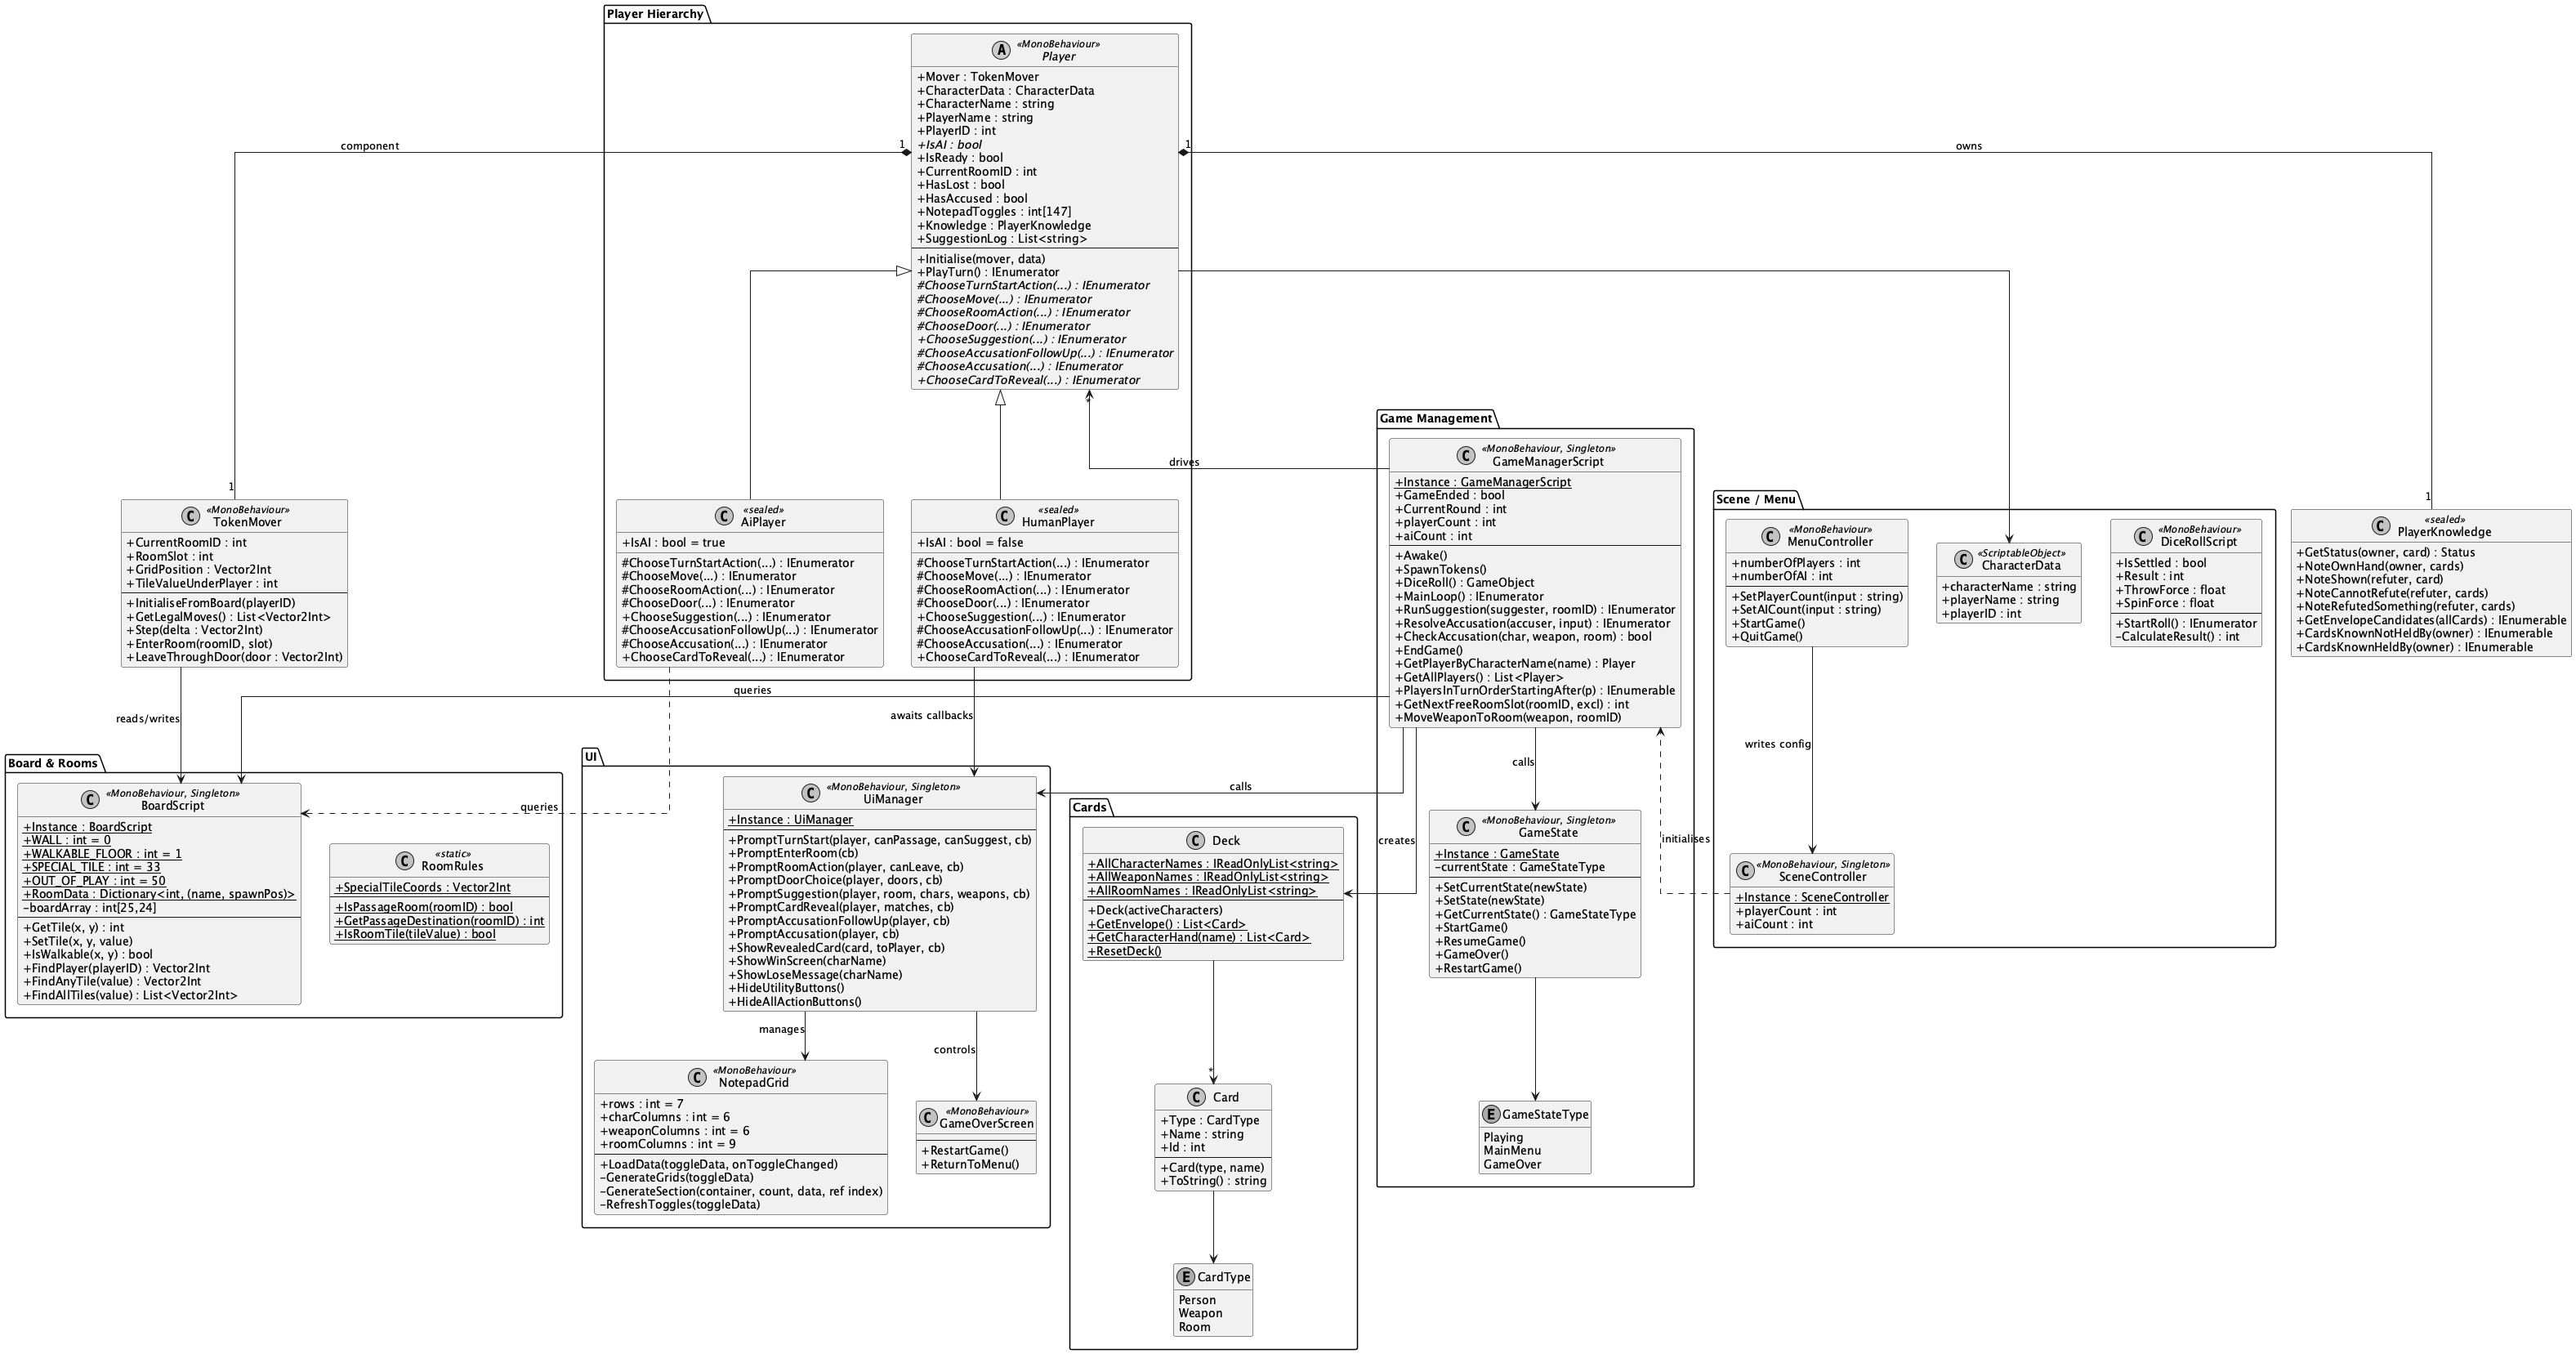
\includegraphics[width=\textwidth]{class_diagram.png}
\caption{Full class diagram --- all sprints}
\label{fig:class-diagram}
\end{figure}

\textbf{cards.json structure:}
\begin{verbatim}
{
  "names":   ["Miss Scarlett","Colonel Mustard","Mrs. White",
              "Reverend Green","Mrs. Peacock","Professor Plum"],
  "weapons": ["Candlestick","Dagger","Lead Pipe",
              "Revolver","Rope","Spanner"],
  "rooms":   ["Kitchen","Ballroom","Conservatory","Billiard Room",
              "Library","Study","Hall","Lounge","Dining Room"]
}
\end{verbatim}

\subsection*{Test Plan and Evidence of Testing}

\textbf{Unit Tests:}
\begin{table}[H]
\centering
\resizebox{\textwidth}{!}{%
\begin{tabular}{|l|l|p{5cm}|p{3cm}|p{2.5cm}|l|}
\hline
\textbf{Ref} & \textbf{Class} & \textbf{Description} & \textbf{Expected} & \textbf{Actual} & \textbf{Pass/Fail} \\ \hline
U1.1 & Card & Constructor sets type correctly & card.Type == Person & Person & Pass \\ \hline
U1.2 & Card & ToString() returns name & ``Dagger'' & ``Dagger'' & Pass \\ \hline
U1.3 & Deck & 18 cards dealt after envelope & 18 dealt, 3 in envelope & 18 dealt, 3 in envelope & Pass \\ \hline
U1.4 & Deck & Envelope has one of each type & 1 Person + 1 Weapon + 1 Room & Confirmed & Pass \\ \hline
U1.5 & Deck & GetCharacterHand correct & Non-empty, no duplicates & All verified & Pass \\ \hline
U1.6 & SceneController & Singleton prevents duplicate & Second instance destroyed & Destroyed & Pass \\ \hline
\end{tabular}%
}
\end{table}

\subsection*{Sprint Retrospective}

\textbf{Did you achieve your objectives?} Yes. Unity/C\# agreed and confirmed running on every machine. Deck, Card, and CardType implemented and unit-tested. \texttt{cards.json} in place. \texttt{SceneController} persists player and AI count between scenes.

\textbf{Is there a working prototype?} Not yet a playable game. The project compiles and runs cleanly; card and deck logic is functional.

\textbf{What went well?}
\begin{itemize}
    \item Role split agreed quickly at Meeting 3 before any code was written.
    \item JSON-driven card system designed early, giving downstream systems a fixed data contract.
    \item Edward's early Unity spike de-risked the tool chain from day one.
\end{itemize}

\textbf{What did not go well?}
\begin{itemize}
    \item Repository tooling (Git LFS, Unity merge settings, PR templates) not yet in place --- caused early Sprint 2 conflicts.
    \item Class diagram was rough at sprint close; refined in parallel with implementation.
\end{itemize}

\textbf{What will you do differently?} Front-load repository tooling at the start of Sprint 2: Git LFS, \texttt{.gitattributes}, UnityYAMLMerge, PR templates, Unity compile-check workflow.

% ---- SPRINT 2 ----
\section{Sprint 2 --- Board, Game Manager, Dice \& Scene Infrastructure}
\label{sec:sprint2}

\subsection*{Summary Data}
\begin{tabular}{ll}
\textbf{Team Number:} & 15 \\
\textbf{Sprint Technical Lead:} & Ewan (GameManagerScript + GameState) \\
\textbf{Start Date:} & 05 March 2026 \\
\textbf{End Date:} & 17 March 2026 \\
\end{tabular}

\subsection*{Individual Key Contributions}
\begin{table}[H]
\centering
\resizebox{\textwidth}{!}{%
\begin{tabular}{|l|p{10cm}|}
\hline
\textbf{Team Member} & \textbf{Key Contribution(s)} \\ \hline
Matt & \texttt{BoardScript}: 25-row $\times$ 24-col tile array; walkable, door, player-start squares; board prefab \\ \hline
Ewan & \texttt{GameManagerScript}: singleton, deck init, token spawning, character-order turn loop; \texttt{GameState}: Playing/MainMenu/GameOver state machine \\ \hline
Joe & \texttt{Player} base class: initial tile-position fields and structure; occupancy tracking \\ \hline
Ethan & Board movement planning; room connectivity and door position verification \\ \hline
Ben & \texttt{DiceRollScript}: Rigidbody physics dice; face-orientation result calculation \\ \hline
Edward & \texttt{MenuController}: OnNewGame/QuitGame; wiring \texttt{SceneController} into menu flow \\ \hline
\end{tabular}%
}
\end{table}

\subsection*{Requirements Analysis}

\textbf{Functional Requirements (Mandatory):}
\begin{itemize}
    \item \textbf{F2.1} Board is a 25-row $\times$ 24-col grid. Tile encoding: 0 = wall, 1 = corridor, 2--11 = room door squares, 33 = special tile, 50--55 = player starting positions.
    \item \textbf{F2.2} Game initialises automatically: board rendered, tokens spawned, deck with murder envelope created.
    \item \textbf{F2.3} Game supports 2--6 players (human or AI) as configured in the menu.
    \item \textbf{F2.4} Dice produces a result between 1 and 6 inclusive; physics-based.
    \item \textbf{F2.5} Each player token spawns at its designated starting position.
    \item \textbf{F2.6} Game has distinct states: Playing, MainMenu, GameOver.
\end{itemize}

\subsection*{Key Design Decision: Board Tile Encoding}

\begin{table}[H]
\centering
\caption{BoardScript Tile Encoding}
\begin{tabular}{|c|l|}
\hline
\textbf{Value} & \textbf{Meaning} \\ \hline
0 & Wall / impassable \\ \hline
1 & Walkable corridor (\texttt{WALKABLE\_FLOOR}) \\ \hline
2--11 & Room door entry square (value = room ID) \\ \hline
33 & Special tile (\texttt{SPECIAL\_TILE}) \\ \hline
50--55 & Player starting positions (\texttt{OCCUPIED = 50}) \\ \hline
\end{tabular}
\end{table}

\textbf{Room ID Mapping} (\texttt{BoardScript.RoomData}):

\begin{table}[H]
\centering
\caption{Room ID to Name Mapping }
\begin{tabular}{|c|l|}
\hline
\textbf{ID} & \textbf{Room} \\ \hline
2 & Study \\ \hline
3 & Hall \\ \hline
4 & Lounge \\ \hline
5 & Library \\ \hline
6 & Dining Room \\ \hline
7 & Billiard Room \\ \hline
8 & Conservatory \\ \hline
9 & Ballroom \\ \hline
10 & Kitchen \\ \hline
11 & Stairwell \\ \hline
\end{tabular}
\end{table}

\subsection*{Key Design Decision: Physics Dice}

A Rigidbody physics dice was chosen over \texttt{Random.Range(1,7)} to provide visual authenticity (Watson Games requirement: ``fun to play, colourful interface''). \texttt{CalculateResult()} uses dot products against \texttt{Vector3.up} to identify the uppermost face. A \texttt{Random.Range(1,7)} fallback is used if no face is clearly detected.

\subsection*{Test Plan and Evidence of Testing}

\textbf{Unit Tests:}
\begin{table}[H]
\centering
\resizebox{\textwidth}{!}{%
\begin{tabular}{|l|l|p{5cm}|p{3cm}|p{2.5cm}|l|}
\hline
\textbf{Ref} & \textbf{Class} & \textbf{Description} & \textbf{Expected} & \textbf{Actual} & \textbf{Pass/Fail} \\ \hline
U2.1 & BoardScript & GetTile returns 0 for out-of-bounds coordinates & 0 & 0 & Pass \\ \hline
U2.2 & BoardScript & GetTile returns 1 for known corridor tile (7,0) & 1 & 1 & Pass \\ \hline
U2.3 & BoardScript & IsWalkable returns false for wall tile (value 0) & false & false & Pass \\ \hline
U2.4 & BoardScript & IsWalkable returns true for door tile (value 2) & true & true & Pass \\ \hline
U2.5 & DiceRollScript & CalculateResult returns value in range 1--6 for all 6 face orientations & 1 $\leq$ result $\leq$ 6 & All 6 orientations in range & Pass \\ \hline
U2.6 & GameManagerScript & Singleton prevents duplicate instance & Second instance destroyed & Second destroyed & Pass \\ \hline
U2.7 & GameState & SetCurrentState(GameOver) sets timeScale to 0 & timeScale = 0 & timeScale = 0 & Pass \\ \hline
\end{tabular}%
}
\end{table}

\textbf{System Tests:}
\begin{table}[H]
\centering
\resizebox{\textwidth}{!}{%
\begin{tabular}{|l|l|p{4cm}|p{3cm}|p{3cm}|l|}
\hline
\textbf{Ref} & \textbf{Req} & \textbf{Description} & \textbf{Expected} & \textbf{Actual} & \textbf{P/F} \\ \hline
S2.1 & F2.2 & Game starts and board renders & Board visible; no errors & Board renders; console clean & Pass \\ \hline
S2.2 & F2.5 & Tokens spawn correctly & Tokens at start squares & Tokens at correct positions & Pass \\ \hline
S2.3 & F2.4 & Dice gives valid result & Value 1--6 & 1--6 displayed & Pass \\ \hline
S2.4 & F2.6 & Menu transitions to game scene & Scene loads with correct count & Scene transition works & Pass \\ \hline
\end{tabular}%
}
\end{table}

\subsection*{Sprint Retrospective}

\textbf{Did you achieve your objectives?} Yes. \texttt{BoardScript} with 25-row $\times$ 24-col tile encoding is in place. \texttt{GameManagerScript} handles player setup and deck initialisation. \texttt{DiceRollScript} produces physics-based rolls. Tokens spawn at designated start positions.

\textbf{What went well?}
\begin{itemize}
    \item Repository tooling (Git LFS, \texttt{.gitattributes}, UnityYAMLMerge, PR templates, Unity compile-check) completed in week 1 of Sprint 2 --- prevented destructive merge conflicts for the remainder of the project (R2 mitigated).
    \item Singleton patterns for \texttt{GameManagerScript}, \texttt{BoardScript}, and \texttt{GameState} made cross-script communication clean and predictable.
    \item Matt's Unity walkthrough at Meeting 5 levelled-up backend-focused team members.
\end{itemize}

\textbf{What did not go well?}
\begin{itemize}
    \item Repo tooling consumed $\sim$1 week of effort not budgeted in the Gantt.
    \item The deck refactor briefly delayed GameManager work ($\sim$2 days).
\end{itemize}

\textbf{What will you do differently?} Begin \texttt{TokenMovementScript} with a clearly bounded scope --- legal-move detection only, not A* pathfinding. Schedule the Easter break explicitly in Sprint 3 plan. Adopt \texttt{Vector2Int} as the standard board-coordinate type from day one of Sprint 3.

% ---- SPRINT 3 ----
\section{Sprint 3 --- Movement, Rooms, UI \& Detective Notebook}
\label{sec:sprint3}

\subsection*{Summary Data}
\begin{tabular}{ll}
\textbf{Team Number:} & 15 \\
\textbf{Sprint Technical Lead:} & Joe (movement lead, paired with Ethan) \\
\textbf{Start Date:} & 17 March 2026 \\
\textbf{End Date:} & 11 April 2026 \\
\end{tabular}

\subsection*{Individual Key Contributions}
\begin{table}[H]
\centering
\resizebox{\textwidth}{!}{%
\begin{tabular}{|l|p{10cm}|}
\hline
\textbf{Team Member} & \textbf{Key Contribution(s)} \\ \hline
Joe & \texttt{Player}/\texttt{HumanPlayer}/\texttt{TokenMover}: legal-move detection, keyboard input, room-entry detection \\ \hline
Ethan & \texttt{TokenMover} support: board occupancy rules, movement edge-case testing \\ \hline
Ewan & \texttt{Player} base class turn coroutine (\texttt{PlayTurn}); \texttt{WaitUntil} async UI patterns \\ \hline
Matt & \texttt{UiManager} singleton; all turn-prompt/suggestion/card-reveal UI; \texttt{NotepadGrid} (\texttt{NotepadUI.cs}); \texttt{GameOverScreen} \\ \hline
Ben & \texttt{RoomRules}: secret passage map; passage room detection \\ \hline
Edward & \texttt{CharacterData} ScriptableObject; JSON integration verification \\ \hline
\end{tabular}%
}
\end{table}

\subsection*{Key Design Decision: Player Class Hierarchy}

The original \texttt{TokenMovementScript} concept was refactored into a clean class hierarchy that separates movement mechanics from game-logic decisions:

\begin{itemize}
    \item \textbf{\texttt{Player} (abstract MonoBehaviour):} owns all turn sequencing (\texttt{PlayTurn} coroutine), board-position state delegation, knowledge tracking (\texttt{PlayerKnowledge}), and notepad toggles. Defines abstract ``decision hook'' methods that subclasses override.
    \item \textbf{\texttt{HumanPlayer}:} overrides decision hooks by calling \texttt{UiManager} and awaiting player input.
    \item \textbf{\texttt{AiPlayer}:} overrides decision hooks: BFS-directed movement toward envelope-candidate rooms, knowledge-filtered suggestions, and envelope-based accusation trigger (satisfies Watson Games AI requirement).
    \item \textbf{\texttt{TokenMover} (MonoBehaviour component on the same prefab):} handles all grid movement, room entry/exit, and world-space positioning. Exposes \texttt{GetLegalMoves()}, \texttt{Step()}, \texttt{EnterRoom()}, \texttt{LeaveThroughDoor()}.
\end{itemize}

\subsection*{Key Design Decision: Legal Move Detection (Not A* Pathfinding)}

\texttt{TokenMover.GetLegalMoves()} returns the set of immediately adjacent walkable tiles (orthogonal only). The player selects direction step-by-step. This matches the Clue! rules and avoids over-engineering. A* pathfinding was cut at Meeting 6 once the irregular-board complexity was understood.

\subsection*{Key Design Decision: Callback-Driven UI}

\texttt{UiManager} communicates results to game logic via \texttt{System.Action} delegates; \texttt{Player} coroutines wait via \texttt{WaitUntil}. This keeps UI code and game logic separated: the turn coroutine does not need to know how the UI is implemented.

\subsection*{Secret Passages (\texttt{RoomRules})}

Secret passages are implemented in the static \texttt{RoomRules} class:
\begin{itemize}
    \item Study (ID 2) $\leftrightarrow$ Kitchen (ID 10)
    \item Lounge (ID 4) $\leftrightarrow$ Conservatory (ID 8)
\end{itemize}
A player in a passage room can take \texttt{TurnAction.Passage} instead of rolling.

\subsection*{NotepadGrid}

\texttt{NotepadGrid} (in \texttt{NotepadUI.cs}) generates three toggle sections for characters, weapons, and rooms. Section dimensions are configured via Unity Inspector fields (\texttt{charColumns=6}, \texttt{weaponColumns=6}, \texttt{roomColumns=9}, \texttt{rows=7}). Toggle state is stored as \texttt{int[147]} in \texttt{Player.NotepadToggles} (7 rows $\times$ 6 characters + 7 rows $\times$ 6 weapons + 7 rows $\times$ 9 rooms = 147 cells).

\subsection*{Sequence Diagram --- Player Turn (Movement Phase)}

\begin{figure}[H]
\centering
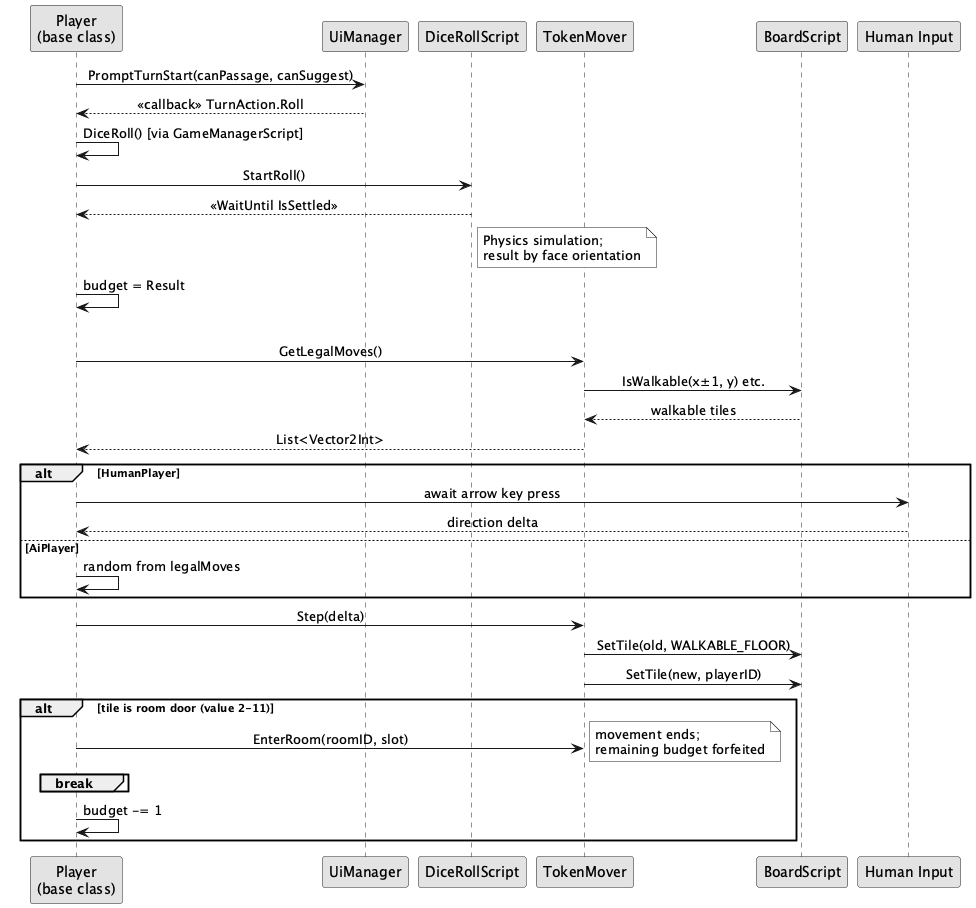
\includegraphics[width=\textwidth]{sequence_movement.png}
\caption{Sequence diagram --- player turn movement phase}
\label{fig:seq-movement}
\end{figure}

\subsection*{Test Plan and Evidence of Testing}

\textbf{Unit Tests:}
\begin{table}[H]
\centering
\resizebox{\textwidth}{!}{%
\begin{tabular}{|l|l|p{5cm}|p{3cm}|p{2.5cm}|l|}
\hline
\textbf{Ref} & \textbf{Class} & \textbf{Description} & \textbf{Expected} & \textbf{Actual} & \textbf{Pass/Fail} \\ \hline
U3.1 & TokenMover & Legal moves exclude impassable (value 0) tiles & 0-tile not in result & 0-tile excluded & Pass \\ \hline
U3.2 & TokenMover & Legal moves exclude out-of-play (value $\geq$ 50) tiles & $\geq$50 tile not in result & Excluded & Pass \\ \hline
U3.3 & RoomRules & IsRoomTile returns true for door values (2, 5, 9, 11); false for non-door values & true/false per value & All cases correct & Pass \\ \hline
U3.4 & BoardScript & Tile resets to WALKABLE\_FLOOR (1) after token steps away & Old tile = 1 & Old tile reset to 1 & Pass \\ \hline
U3.5 & BoardScript & RoomData maps room IDs 2--11 to correct room names & e.g.\ RoomData[2].name = ``Study'' & All 10 room names correct & Pass \\ \hline
U3.6 & NotepadGrid & LoadData processes 147 toggles (21 columns $\times$ 7 rows) & Toggle count = 147 & 147 toggles & Pass \\ \hline
\end{tabular}%
}
\end{table}

\textbf{System Tests:}
\begin{table}[H]
\centering
\resizebox{\textwidth}{!}{%
\begin{tabular}{|l|l|p{4cm}|p{3cm}|p{3cm}|l|}
\hline
\textbf{Ref} & \textbf{Req} & \textbf{Description} & \textbf{Expected} & \textbf{Actual} & \textbf{P/F} \\ \hline
S3.1 & F3.1 & Player moves by dice value & Token moves N squares & Moves exactly N & Pass \\ \hline
S3.2 & F3.2 & Diagonal movement blocked & Only orthogonal & Diagonal ignored & Pass \\ \hline
S3.3 & F3.3 & Two tokens cannot share corridor & Move blocked & Blocked & Pass \\ \hline
S3.4 & F3.4 & Room entry ends movement & Movement stops & Halts on door tile & Pass \\ \hline
S3.5 & F3.6 & Turn UI appears on player turn & Controls visible & UiManager prompts & Pass \\ \hline
S3.6 & F3.7 & Suggestion UI shows correct room & Room field locked & Read-only field & Pass \\ \hline
S3.7 & F3.9 & AI moves without input & AI selects move & Turn completes & Pass \\ \hline
\end{tabular}%
}
\end{table}

\subsection*{Sprint Retrospective}

\textbf{Did you achieve your objectives?} Partially. \texttt{Player}/\texttt{HumanPlayer}/\texttt{AiPlayer}/\texttt{TokenMover}, \texttt{RoomRules}, \texttt{UiManager}, and \texttt{NotepadGrid} were delivered. A* pathfinding was scoped down to legal-move-only detection. Suggestion/Accusation was formally pushed into Sprint 4 at Meeting 8.

\textbf{What went well?}
\begin{itemize}
    \item The Player class hierarchy cleanly separates game logic from rendering and input.
    \item \texttt{UiManager} as single UI entry point kept GUI logic decoupled from movement and game-state code.
    \item \texttt{Vector2Int} adopted as standard at Meeting 7, avoiding coordinate-system bugs in Sprint 4.
\end{itemize}

\textbf{What did not go well?}
\begin{itemize}
    \item Easter break (20 March -- 14 April) paused all development for $\sim$3.5 weeks.
    \item Legal-move detection on the irregular Cluedo board was more complex than estimated.
    \item Suggestion/Accusation (originally Sprint 3 work) deferred into Sprint 4, compressing that sprint.
\end{itemize}

\textbf{What will you do differently?} Focus Sprint 4 exclusively on the end-to-end game loop. Plan a single integration day mid-sprint. Accept architectural compromises where a refactor risks the deadline.

% ---- SPRINT 4 ----
\section{Sprint 4 --- Game Loop, Suggestions, Accusations \& Testing}
\label{sec:sprint4}

\subsection*{Summary Data}
\begin{tabular}{ll}
\textbf{Team Number:} & 15 \\
\textbf{Sprint Technical Lead:} & Ewan (MainLoop, Suggestion, Accusation) \\
\textbf{Start Date:} & 11 April 2026 \\
\textbf{End Date:} & 30 April 2026 \\
\end{tabular}

\subsection*{Individual Key Contributions}
\begin{table}[H]
\centering
\resizebox{\textwidth}{!}{%
\begin{tabular}{|l|p{10cm}|}
\hline
\textbf{Team Member} & \textbf{Key Contribution(s)} \\ \hline
Ewan & \texttt{GameManagerScript.MainLoop()}: full coroutine turn cycle; \texttt{RunSuggestion()}: clockwise card-showing; \texttt{ResolveAccusation()} \\ \hline
Ben & \texttt{AiPlayer} decision methods: BFS-directed move, knowledge-filtered suggestion, envelope-based accusation \\ \hline
Joe & \texttt{Player.DoSuggestionThenAccusation()}: room-entry suggestion + accusation follow-up \\ \hline
Ethan & Movement edge cases; room entry integration testing; large-branch merge \\ \hline
Matt & \texttt{GameOverScreen}: restart / return-to-menu; final UI polish \\ \hline
Edward & \texttt{MenuController} input wiring; \texttt{PlayerKnowledge} integration; documentation \\ \hline
\end{tabular}%
}
\end{table}

\subsection*{Requirements Analysis}

\textbf{Functional Requirements (Mandatory):}
\begin{itemize}
    \item \textbf{F4.1} Turn order: Miss Scarlett, Colonel Mustard, Mrs. White, Reverend Green, Mrs. Peacock, Professor Plum.
    \item \textbf{F4.2} Suggestion only available when token is in a room.
    \item \textbf{F4.3} Suggestion room is fixed as the player's current room.
    \item \textbf{F4.4} Clockwise card-showing round: each player reveals one matching card if held; first match ends the round.
    \item \textbf{F4.5} Suggested character token is moved into the suggestion room (\texttt{target.Mover.EnterRoom()}).
    \item \textbf{F4.6} Accusation checks three chosen cards against the murder envelope (\texttt{Deck.GetEnvelope()}).
    \item \textbf{F4.7} Correct accusation triggers win/game-over state.
    \item \textbf{F4.8} Incorrect accusation eliminates the player; their hand remains for suggestion responses.
    \item \textbf{F4.9} AI player completes a full turn without human input.
\end{itemize}

\subsection*{Key Design Decision: Suggestion and Accusation in GameManagerScript}

The original design called for standalone \texttt{Suggestion} and \texttt{Accusation} classes. Under time pressure in Sprint 4, both were implemented directly in \texttt{GameManagerScript}:

\begin{itemize}
    \item \texttt{GameManagerScript.RunSuggestion()} --- coroutine that iterates players clockwise, prompts card reveal, updates \texttt{PlayerKnowledge}, logs refutations, and calls \texttt{UiManager.ShowRevealedCard()} for private display.
    \item \texttt{GameManagerScript.ResolveAccusation()} --- checks accusation against \texttt{Deck.GetEnvelope()}, calls \texttt{EndGame()} on correct or sets \texttt{player.HasLost = true} on incorrect.
\end{itemize}

This is a known architectural deviation (KI-4), documented transparently.

\subsection*{Key Design Decision: PlayerKnowledge}

A \texttt{PlayerKnowledge} class was added to track per-player card inferences:
\begin{itemize}
    \item \textbf{Held facts:} cards known to be held by a specific player (from \texttt{NoteShown} or own hand).
    \item \textbf{NotHeld facts:} cards known not held by a player (from \texttt{NoteCannotRefute}).
    \item \textbf{Disjunctions:} a player refuted \textit{something}, but the observer didn't see which card (\texttt{NoteRefutedSomething}).
    \item \textbf{Envelope candidates:} cards not definitively held by anyone (\texttt{GetEnvelopeCandidates()}).
\end{itemize}

\texttt{PlayerKnowledge} is wired into \texttt{GameManagerScript.RunSuggestion()} and exposed to \texttt{AiPlayer} for future deduction logic.

\subsection*{Turn State Machine}

\begin{figure}[H]
\centering
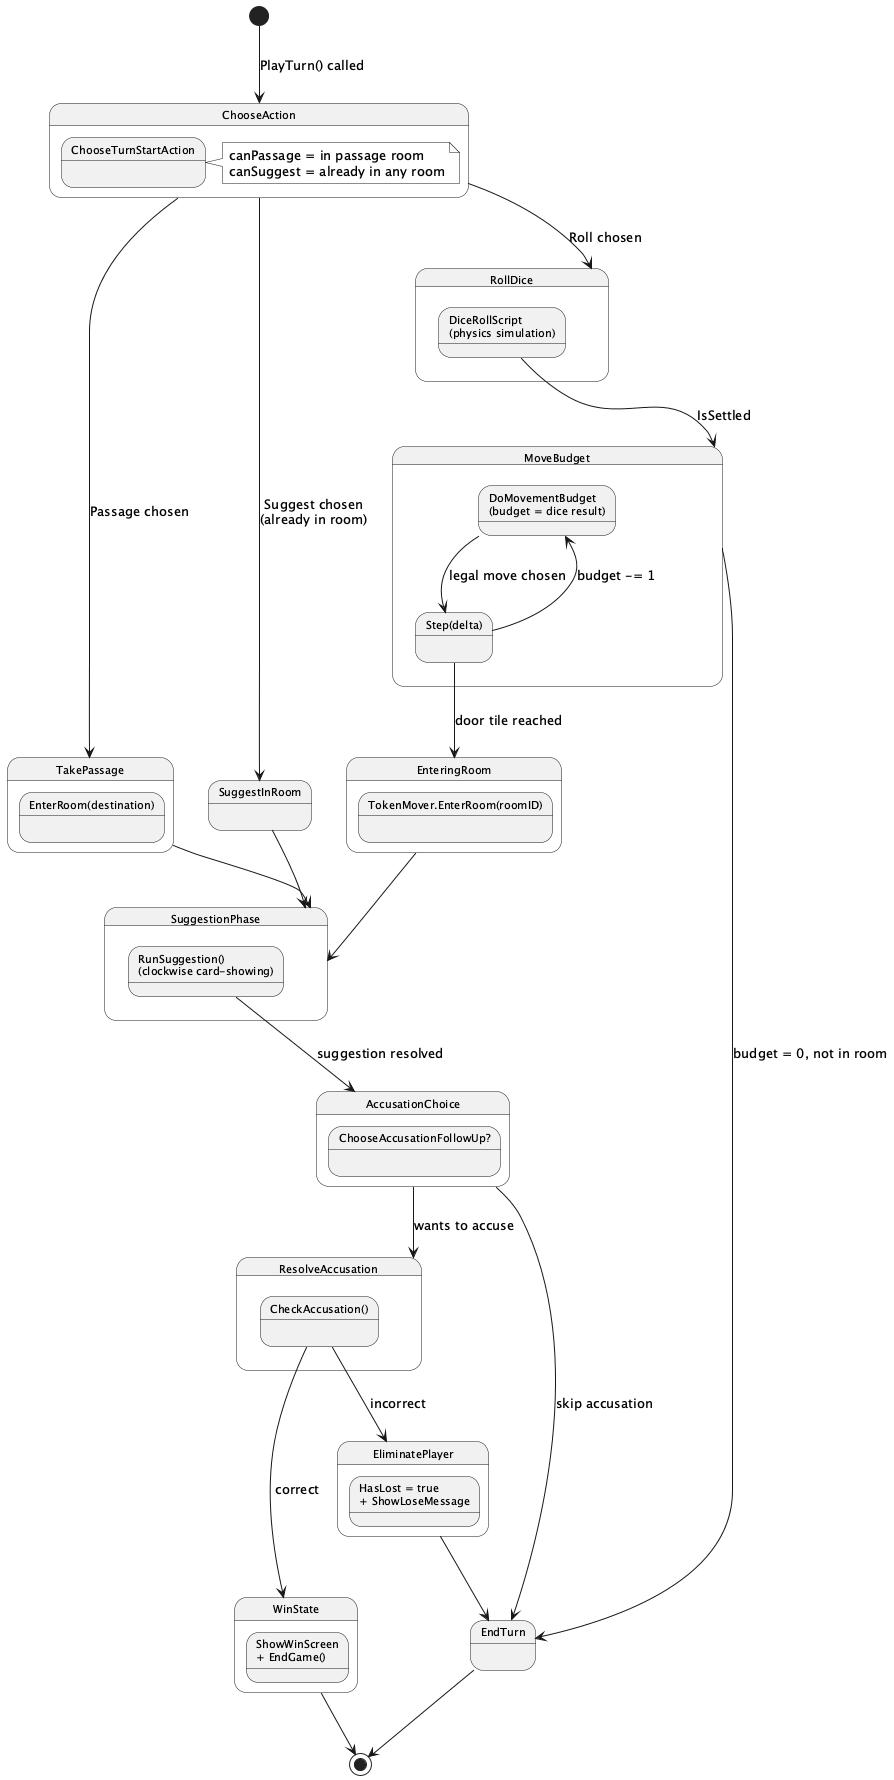
\includegraphics[width=0.85\textwidth]{state_turn.png}
\caption{Turn state machine}
\label{fig:state-turn}
\end{figure}

\subsection*{Sequence Diagram --- Suggestion Resolution}

\begin{figure}[H]
\centering
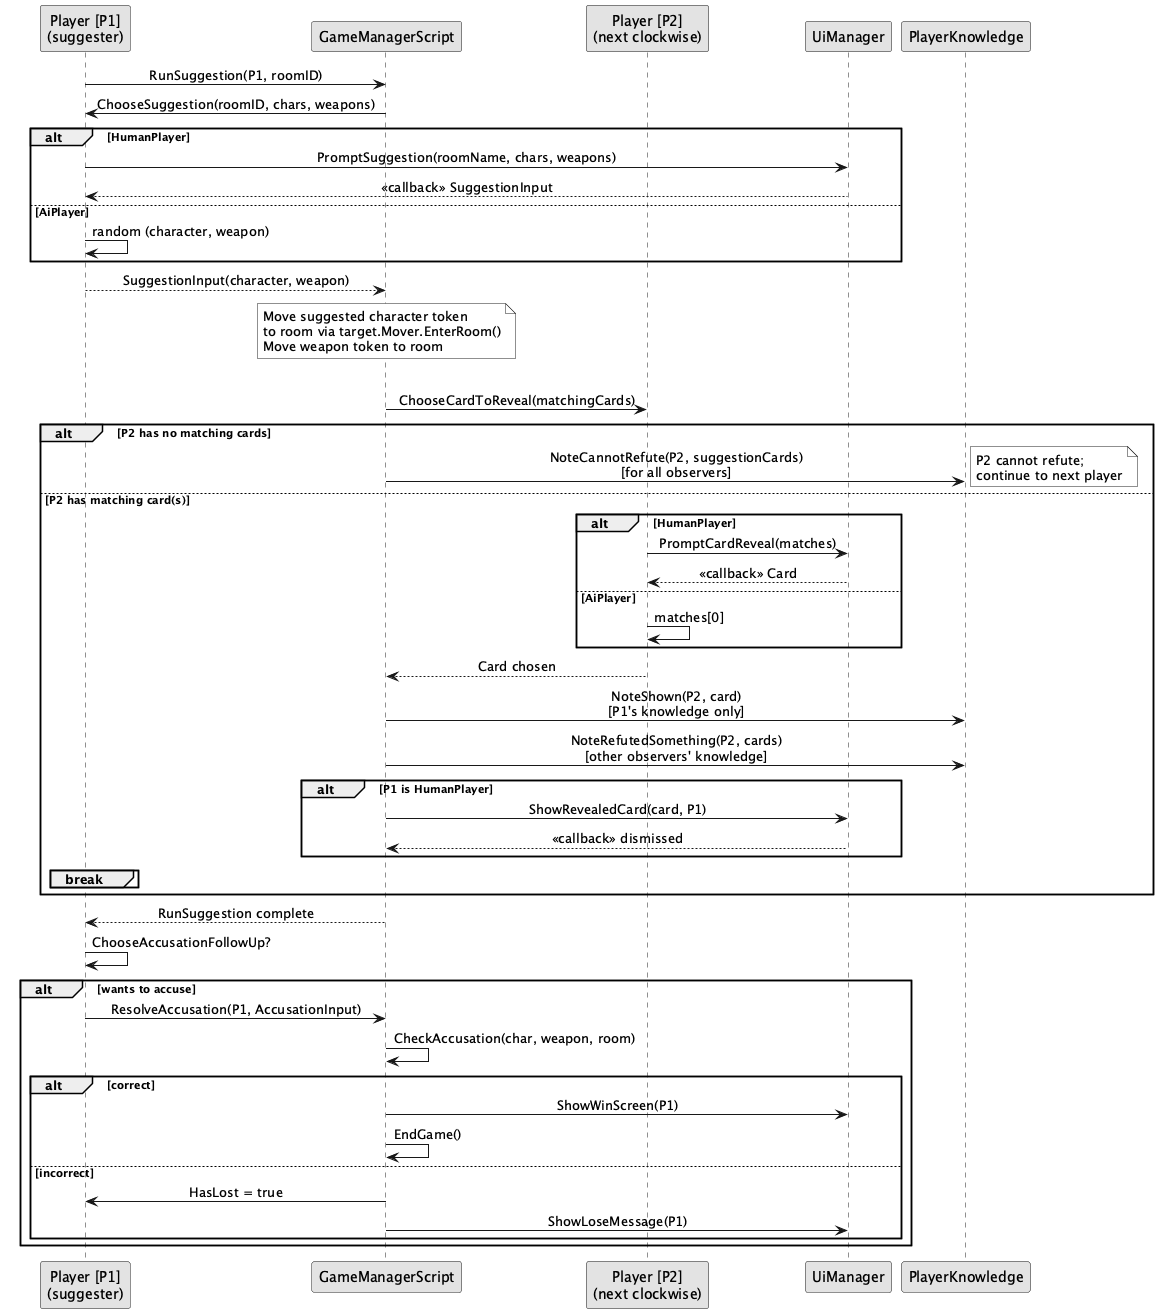
\includegraphics[width=\textwidth]{sequence_suggestion.png}
\caption{Sequence diagram --- suggestion resolution}
\label{fig:seq-suggestion}
\end{figure}

\subsection*{Test Plan and Evidence of Testing}

\textbf{Unit Tests:}
\begin{table}[H]
\centering
\resizebox{\textwidth}{!}{%
\begin{tabular}{|l|l|p{5cm}|p{3cm}|p{2.5cm}|l|}
\hline
\textbf{Ref} & \textbf{Class} & \textbf{Description} & \textbf{Expected} & \textbf{Actual} & \textbf{Pass/Fail} \\ \hline
U4.1 & GameManagerScript & Turn order cycles Scarlett$\to$Mustard$\to$White (canonical character order) & Correct order & Correct order & Pass \\ \hline
U4.2 & GameManagerScript & Player with HasLost=true is excluded from active turn order & Mustard absent from order & Mustard absent & Pass \\ \hline
U4.3 & GameManagerScript & CheckAccusation returns true when all three cards match the envelope & true & true & Pass \\ \hline
U4.4 & GameManagerScript & CheckAccusation returns false for wrong guess; accuser HasLost set true & false; HasLost = true & Confirmed & Pass \\ \hline
U4.5 & GameManagerScript & RunSuggestion: refuter's revealed card recorded as Held in suggester's PlayerKnowledge & Knowledge.Status = Held & Held confirmed & Pass \\ \hline
U4.6 & GameManagerScript & RunSuggestion: SuggestionLog records no-refute when no player holds matching cards & log contains ``could not refute'' & Confirmed & Pass \\ \hline
U4.7 & GameManagerScript & RunSuggestion moves suggested character's CurrentRoomID to suggestion room & CurrentRoomID = targetRoom & \textbf{Failing} --- EnterRoom dependency on BoardScript.Instance in Play Mode & \textbf{Fail} \\ \hline
\end{tabular}%
}
\end{table}

\textbf{System Tests:}

\noindent\textit{Note: the system tests below were designed against functional requirements F4.1--F4.9 and non-functional requirement NF4.2. The test cases and expected outputs were completed, but manual play-through results and Pass/Fail verdicts could not be recorded before the submission deadline. The incomplete Actual and Pass/Fail columns are an acknowledged gap against the 9--10 band for testing documentation (see Marking Scheme).}
\begin{table}[H]
\centering
\resizebox{\textwidth}{!}{%
\begin{tabular}{|l|l|p{4cm}|p{3cm}|p{3cm}|l|}
\hline
\textbf{Ref} & \textbf{Req} & \textbf{Description} & \textbf{Expected} & \textbf{Actual} & \textbf{P/F} \\ \hline
S4.1 & F4.1 & Miss Scarlett goes first & Turn 1 = Scarlett & \textit{[TODO]} & \textit{[TODO]} \\ \hline
S4.2 & F4.1 & Turn order cycles correctly & P1$\to$P2$\to$P3$\to$P1 & \textit{[TODO]} & \textit{[TODO]} \\ \hline
S4.3 & F4.2 & Suggestion unavailable on corridor & No suggestion prompt & \textit{[TODO]} & \textit{[TODO]} \\ \hline
S4.4 & F4.3 & Current room locked in suggestion UI & Room = current room; read-only & \textit{[TODO]} & \textit{[TODO]} \\ \hline
S4.5 & F4.4 & Clockwise card show; first match stops round & P2 reveals to P1; P3 not asked & \textit{[TODO]} & \textit{[TODO]} \\ \hline
S4.6 & F4.4 & No card shown if nobody holds matching cards & No reveal; round ends & \textit{[TODO]} & \textit{[TODO]} \\ \hline
S4.7 & F4.5 & Suggested character token moves to suggestion room & Token in room & \textit{[TODO]} & \textit{[TODO]} \\ \hline
S4.8 & F4.7 & Correct accusation shows win screen & Win screen displayed & \textit{[TODO]} & \textit{[TODO]} \\ \hline
S4.9 & F4.8 & Wrong accusation eliminates player; they still respond to suggestions & Player skipped; still refutes & \textit{[TODO]} & \textit{[TODO]} \\ \hline
S4.10 & F4.8 & Eliminated players are skipped in turn order & Eliminated player gets no turn & \textit{[TODO]} & \textit{[TODO]} \\ \hline
S4.11 & F4.9 & AI completes a full turn without human input & No hang; completes in $<$5 s & \textit{[TODO]} & \textit{[TODO]} \\ \hline
S4.12 & NF4.2 & Card reveal is private; other players cannot see & Private modal; others unaware & \textit{[TODO]} & \textit{[TODO]} \\ \hline
\end{tabular}%
}
\end{table}

\subsection*{Known Issues / Deficiencies}
\label{sec:sprint4-known-issues}

\begin{table}[H]
\centering
\resizebox{\textwidth}{!}{%
\begin{tabular}{|l|p{5cm}|l|p{3.5cm}|}
\hline
\textbf{ID} & \textbf{Description} & \textbf{Severity} & \textbf{Planned Fix} \\ \hline
KI-1 & \texttt{GameManagerScript.Awake()} falls back to \texttt{playerCount=4, aiCount=2} if \texttt{SceneController} is null. Player/AI counts are adjusted via \texttt{StepHumans(int)}/\texttt{StepAI(int)} in \texttt{MenuController} and written to \texttt{SceneController} in \texttt{OnBegin()}, but the fallback path remains. & Medium & Ensure \texttt{SceneController} is always initialised before \texttt{GameManagerScript.Awake()} \\ \hline
KI-2 & \texttt{SpawnTokens()} comment notes issue with fewer than 6 players; AI player selection uses random shuffle across all 6 slots & Medium & Fix loop condition to handle $<$6 players cleanly \\ \hline
KI-3 & \texttt{AiPlayer} uses BFS-directed movement and knowledge-filtered suggestions; \texttt{ChooseAccusationFollowUp} returns true when envelope candidates narrow to exactly 3. Full notebook-based deduction not implemented. & Low & Extend \texttt{PlayerKnowledge} inference to eliminate cards more aggressively \\ \hline
KI-4 & Suggestion/Accusation lives inside \texttt{GameManagerScript} not standalone classes & Low (architectural) & Extract into \texttt{Suggestion}/\texttt{Accusation} classes; add unit tests \\ \hline
KI-5 & Suggested character and weapon tokens do not fully move to the suggestion room under all conditions. \texttt{RunSuggestion()} calls \texttt{target.Mover.EnterRoom()} only when \texttt{GetPlayerByCharacterName()} returns non-null and the target is not the suggester; \texttt{MoveWeaponToRoom()} is called unconditionally. At least one path is not producing the expected result (\texttt{GameManagerScript.cs} lines 334--338). Root cause not isolated before submission deadline. & Medium (functional) & Trace the exact failing path; add a unit test asserting both token positions after \texttt{RunSuggestion()} \\ \hline
\end{tabular}%
}
\end{table}

\subsection*{Sprint Retrospective}

\textbf{Did you achieve your objectives?} Largely yes. The game loop is integrated end-to-end via `GameManagerScript.MainLoop()`. Suggestion with clockwise card-showing is implemented (`ResolveSuggestion`).
          Accusation evaluation and win / elimination logic both work as specified. The AI player takes full turns without human input. Two issues carry into the known deficiencies log: Suggestion and Accusation logic lives inside `GameManagerScript` and `UiManager` rather than as standalone classes (KI-4, architectural), and system testing identified that suggested character and weapon tokens do not fully move to the suggestion room under all conditions (KI-5, functional). Both are documented in the Known Issues / Deficiencies subsection above.

\textbf{Is there a working prototype?} Yes. A full game of Clue! can be played: players take turns, roll dice, move, enter rooms, make suggestions, see cards revealed privately, and make accusations.

\textbf{What went well?}
\begin{itemize}
    \item Every Sprint 4 critical-path objective shipped.
    \item Large merge on 18 April consolidated all feature branches without losing work.
    \item \texttt{PlayerKnowledge} class provides a clean foundation for future AI deduction.
    \item Sprint 4 testing documented all known limitations rather than hiding them.
\end{itemize}

\textbf{What did not go well?}
\begin{itemize}
    \item Suggestion/Accusation could not be extracted into standalone classes (KI-4).
    \item AI player movement and suggestions are functional (BFS navigation, knowledge-filtered suggestions) but full notebook-based deduction was not implemented (KI-3).
    \item Matt missed Meetings 8 and 9, requiring async communication for UI integration decisions.
\end{itemize}

\textbf{What would you do differently?}
\begin{itemize}
    \item Stub the end-to-end game loop in Sprint 1 so that all systems have a spine to plug into.
    \item Treat the Easter break as a Sprint 3 deadline rather than a transparent pause.
    \item Allocate explicit documentation time in each sprint alongside code.
    \item Front-load all repository tooling on day one of Sprint 1.
\end{itemize}

\newpage

\chapter{Design Documentation --- High Level}
\label{chap:design-high}

\section{System Overview}

The Clue! simulation is a desktop game implemented in Unity (C\#). The table below identifies the major subsystems, their key classes, and responsibilities.

\begin{table}[H]
\centering
\footnotesize
\setlength{\tabcolsep}{5pt}
\begin{tabular}{|p{2.5cm}|p{2.8cm}|p{5.5cm}|}
\hline
\textbf{Subsystem} & \textbf{Key Classes} & \textbf{Responsibility} \\ \hline
Scene Management & \texttt{SceneController}, \texttt{MenuController} & Persists player/AI count between menu and game scenes \\ \hline
Game State & \texttt{GameState} & Tracks Playing / MainMenu / GameOver; controls timescale \\ \hline
Board & \texttt{BoardScript} & 25-row $\times$ 24-col tile grid; single source of truth for occupancy and walkability \\ \hline
Card System & \texttt{Card}, \texttt{Deck} & Loads cards from JSON; creates murder envelope; deals hands \\ \hline
Character Data & \texttt{CharacterData} & ScriptableObject storing character metadata (name, ID) \\ \hline
Game Orchestration & \texttt{GameManagerScript} & Spawns tokens; runs \texttt{MainLoop} coroutine; resolves suggestions and accusations \\ \hline
Player Turn (Human) & \texttt{HumanPlayer} & Waits for UI input via UiManager callbacks \\ \hline
Player Turn (AI) & \texttt{AiPlayer} & Uses BFS-directed movement and knowledge-filtered suggestions; accuses when envelope candidates narrow to 3 \\ \hline
Player Base & \texttt{Player} & Abstract base: turn sequencing, knowledge tracking, notepad state \\ \hline
Movement & \texttt{TokenMover} & Grid movement, room entry/exit, world-space positioning \\ \hline
Rooms / Passages & \texttt{RoomRules} & Static class: room tile detection, secret passage map \\ \hline
Dice & \texttt{DiceRollScript} & Physics Rigidbody dice; result by face orientation \\ \hline
UI & \texttt{UiManager} & Central singleton: all player-facing prompts, suggestion/accusation panels, card reveal \\ \hline
Notebook & \texttt{NotepadGrid} & 147-cell toggle grid for detective deduction \\ \hline
Card Knowledge & \texttt{PlayerKnowledge} & Per-player card inference (Held / NotHeld / disjunctions) \\ \hline
End Screen & \texttt{GameOverScreen} & Restart / return-to-menu on game conclusion \\ \hline
\end{tabular}
\end{table}

\section{Use Cases}

Actors: Human Player, AI Player.

\begin{table}[H]
\centering
\small
\begin{tabular}{|l|l|l|}
\hline
\textbf{Use Case} & \textbf{Human Player} & \textbf{AI Player} \\ \hline
Configure game & \checkmark & --- \\ \hline
Roll dice & \checkmark & \checkmark (auto) \\ \hline
Move token & \checkmark (arrows) & \checkmark (BFS) \\ \hline
Use secret passage & \checkmark & \checkmark (if to target) \\ \hline
Enter room & \checkmark & \checkmark \\ \hline
Make suggestion & \checkmark & \checkmark (filtered) \\ \hline
Respond to suggestion & \checkmark & \checkmark (first card) \\ \hline
View hand & \checkmark & --- \\ \hline
Open detective notebook & \checkmark & --- \\ \hline
Make accusation & \checkmark & \checkmark (3 left) \\ \hline
Restart / return to menu & \checkmark & --- \\ \hline
\end{tabular}
\end{table}

\noindent\textit{Note: ``Make Suggestion'' \texttt{<<include>>} ``Respond to Suggestion''; ``Make Accusation'' ends the game (correct) or eliminates the player (incorrect).}

\begin{figure}[H]
\centering
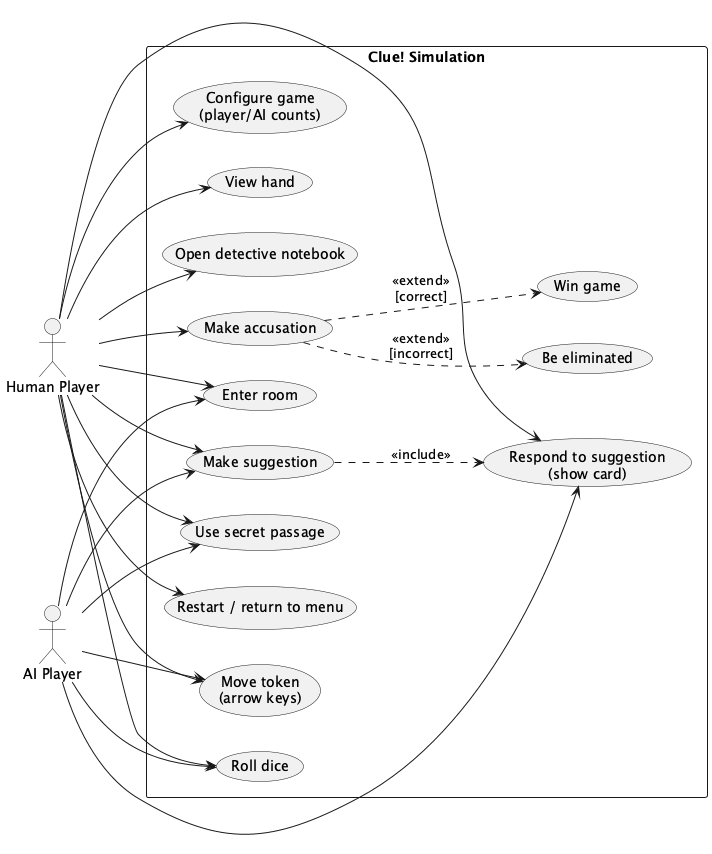
\includegraphics[width=0.85\textwidth]{use_case_diagram.png}
\caption{Use case diagram --- Human Player and AI Player}
\label{fig:use-case}
\end{figure}

\section{Component Interaction Diagram}

\begin{figure}[H]
\centering
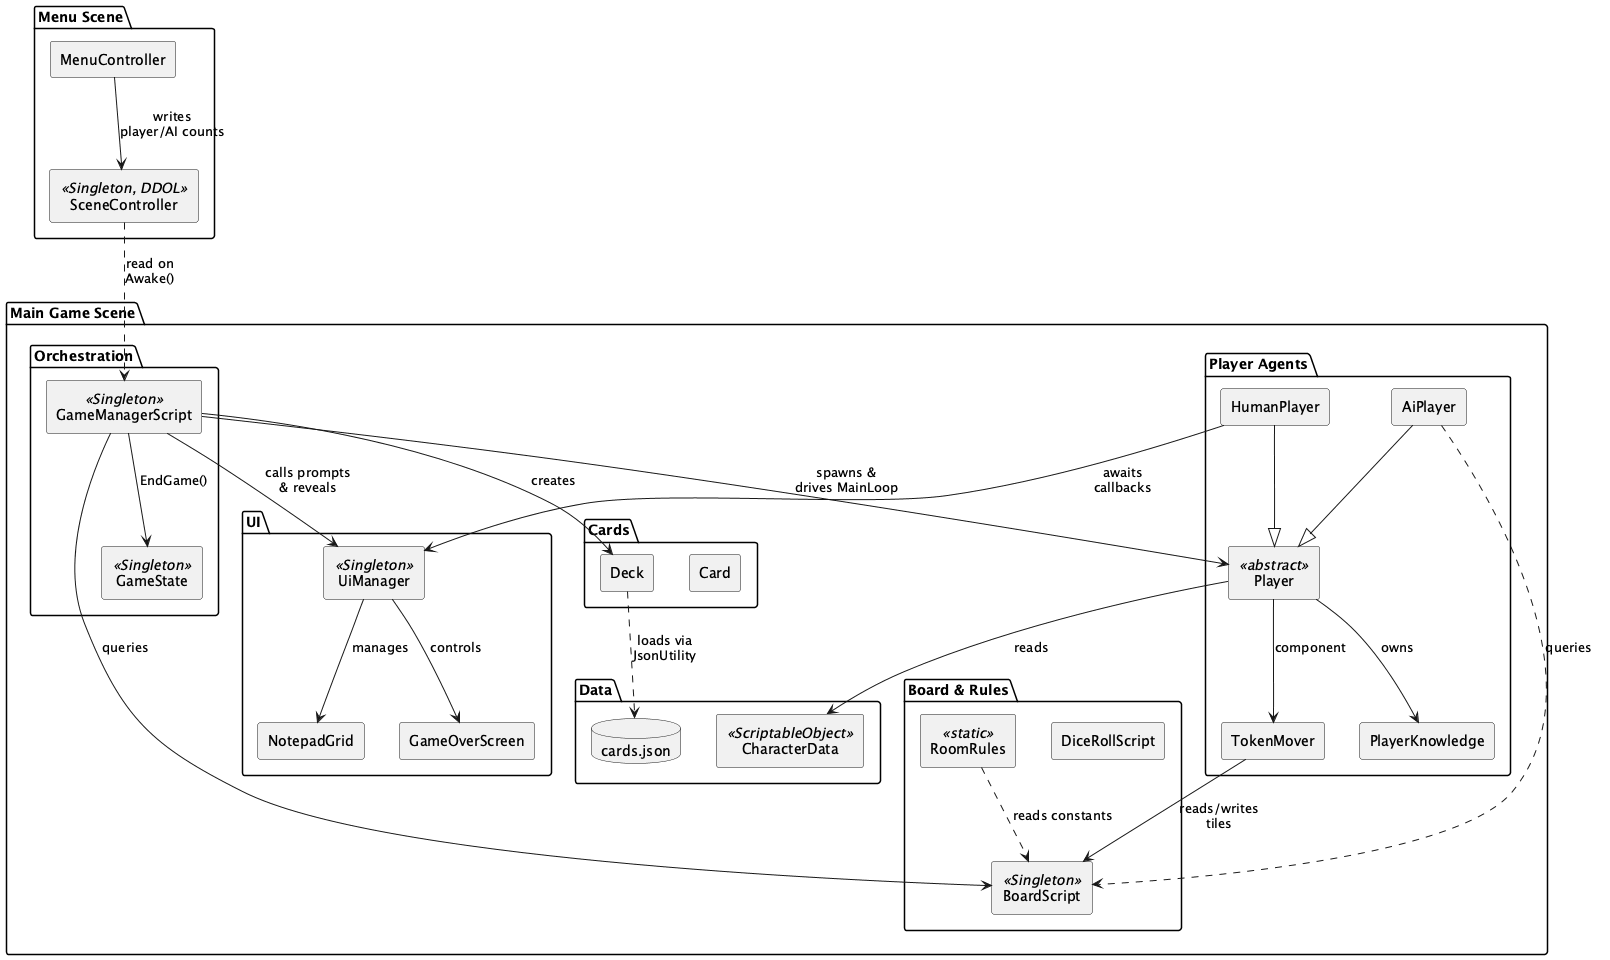
\includegraphics[width=\textwidth]{component_diagram.png}
\caption{Component interaction diagram}
\label{fig:component-diagram}
\end{figure}

\section{Key Design Decisions}

\subsection*{4.1 Unity + C\# (Technology Choice)}
Agreed unanimously at Meeting 1. Unity provides built-in 3D rendering, Rigidbody physics (used for the dice), and cross-platform Mac/PC builds. The team had limited prior Unity experience and saw it as a valuable learning opportunity.

\subsection*{4.2 Singleton Pattern (Manager Classes)}
\texttt{GameManagerScript}, \texttt{BoardScript}, \texttt{UiManager}, \texttt{GameState}, and \texttt{SceneController} all use the Unity Singleton pattern. These represent unique global state that any script may need to access. The singleton prevents duplicate instances and provides a predictable, globally accessible reference.

\subsection*{4.3 Data-Driven Card System}
All card names (characters, weapons, and rooms) are loaded from \texttt{StreamingAssets/cards.json} via \texttt{JsonUtility}. Watson Games explicitly require the game be easily customised. Changing characters or weapons requires only editing this JSON file, with no code changes needed.

\subsection*{4.4 Physics-Based Dice}
\texttt{DiceRollScript} uses a Rigidbody simulation rather than \texttt{Random.Range}. Watson Games require a fun to play and colourful interface, so a physical dice provides visual authenticity. Face orientation is detected by dot product against \texttt{Vector3.up}, and a \texttt{Random.Range(1,7)} fallback handles any degenerate result.

\subsection*{4.5 Callback-Driven UI (Action Delegates)}
\texttt{UiManager} communicates results to game logic via \texttt{System.Action} callbacks, while \texttt{Player} coroutines wait via \texttt{WaitUntil}. This approach keeps UI code and game logic independent.

\subsection*{4.6 AI Player: Basic Decision-Making with Knowledge Scaffold}
\texttt{AiPlayer} uses BFS-directed movement toward envelope-candidate rooms and knowledge-filtered suggestion generation. \texttt{ChooseAccusationFollowUp} returns true when the envelope has been narrowed to exactly 3 candidates. A \texttt{PlayerKnowledge} instance is maintained for each AI player and updated on every suggestion round, providing a foundation for further deduction-based improvements without requiring a rewrite.

\section{Activity Diagram: Full Game Flow}

\begin{figure}[H]
\centering
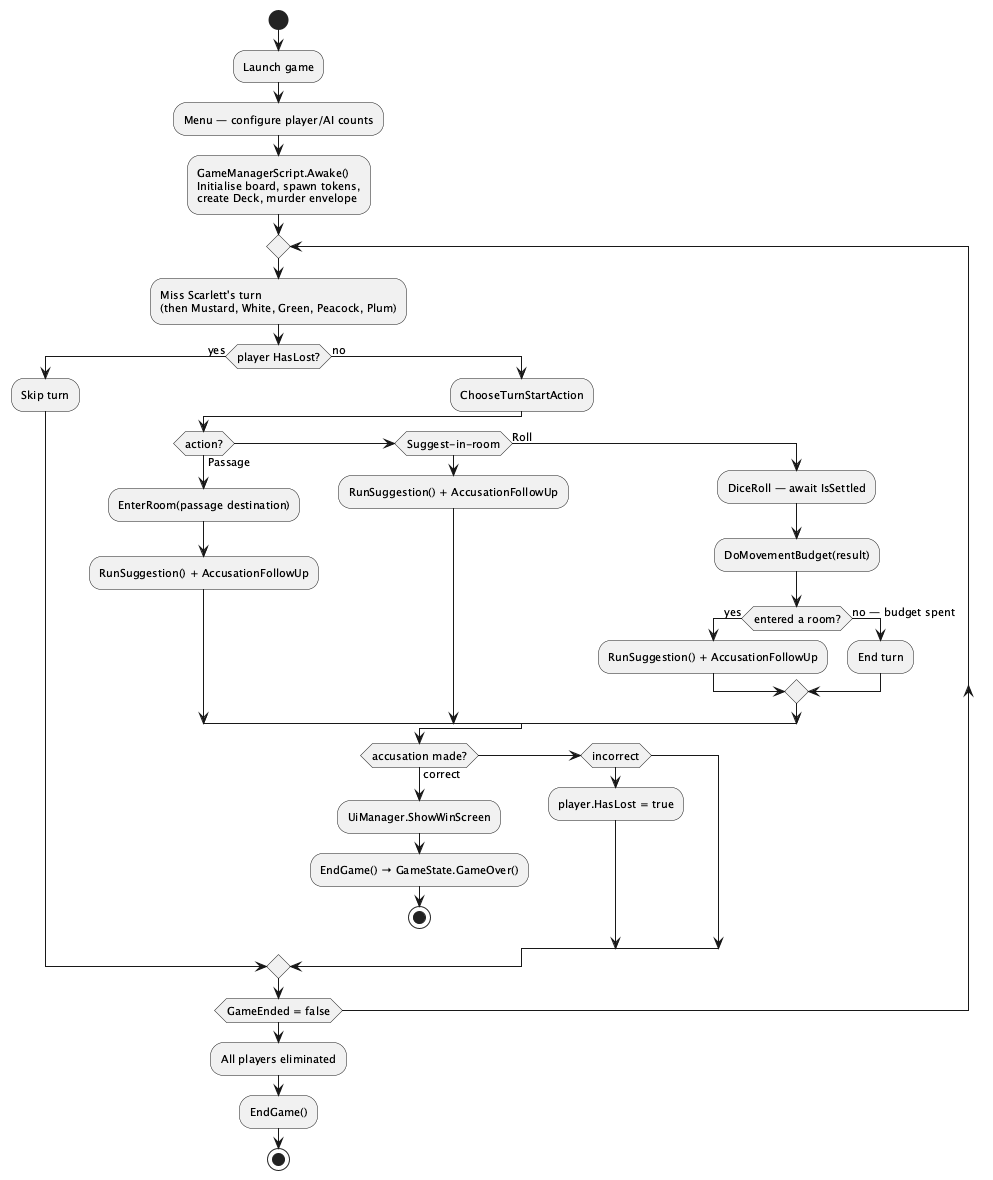
\includegraphics[width=0.75\textwidth]{activity_game_flow.png}
\caption{Activity diagram --- full game flow}
\label{fig:activity-game-flow}
\end{figure}

\newpage

\chapter{Design Documentation: Low Level}
\label{chap:design-low}

\section{Class Diagram}

The full class diagram below shows all major classes, inheritance relationships, aggregation, and key public interfaces.

\begin{figure}[H]
\centering
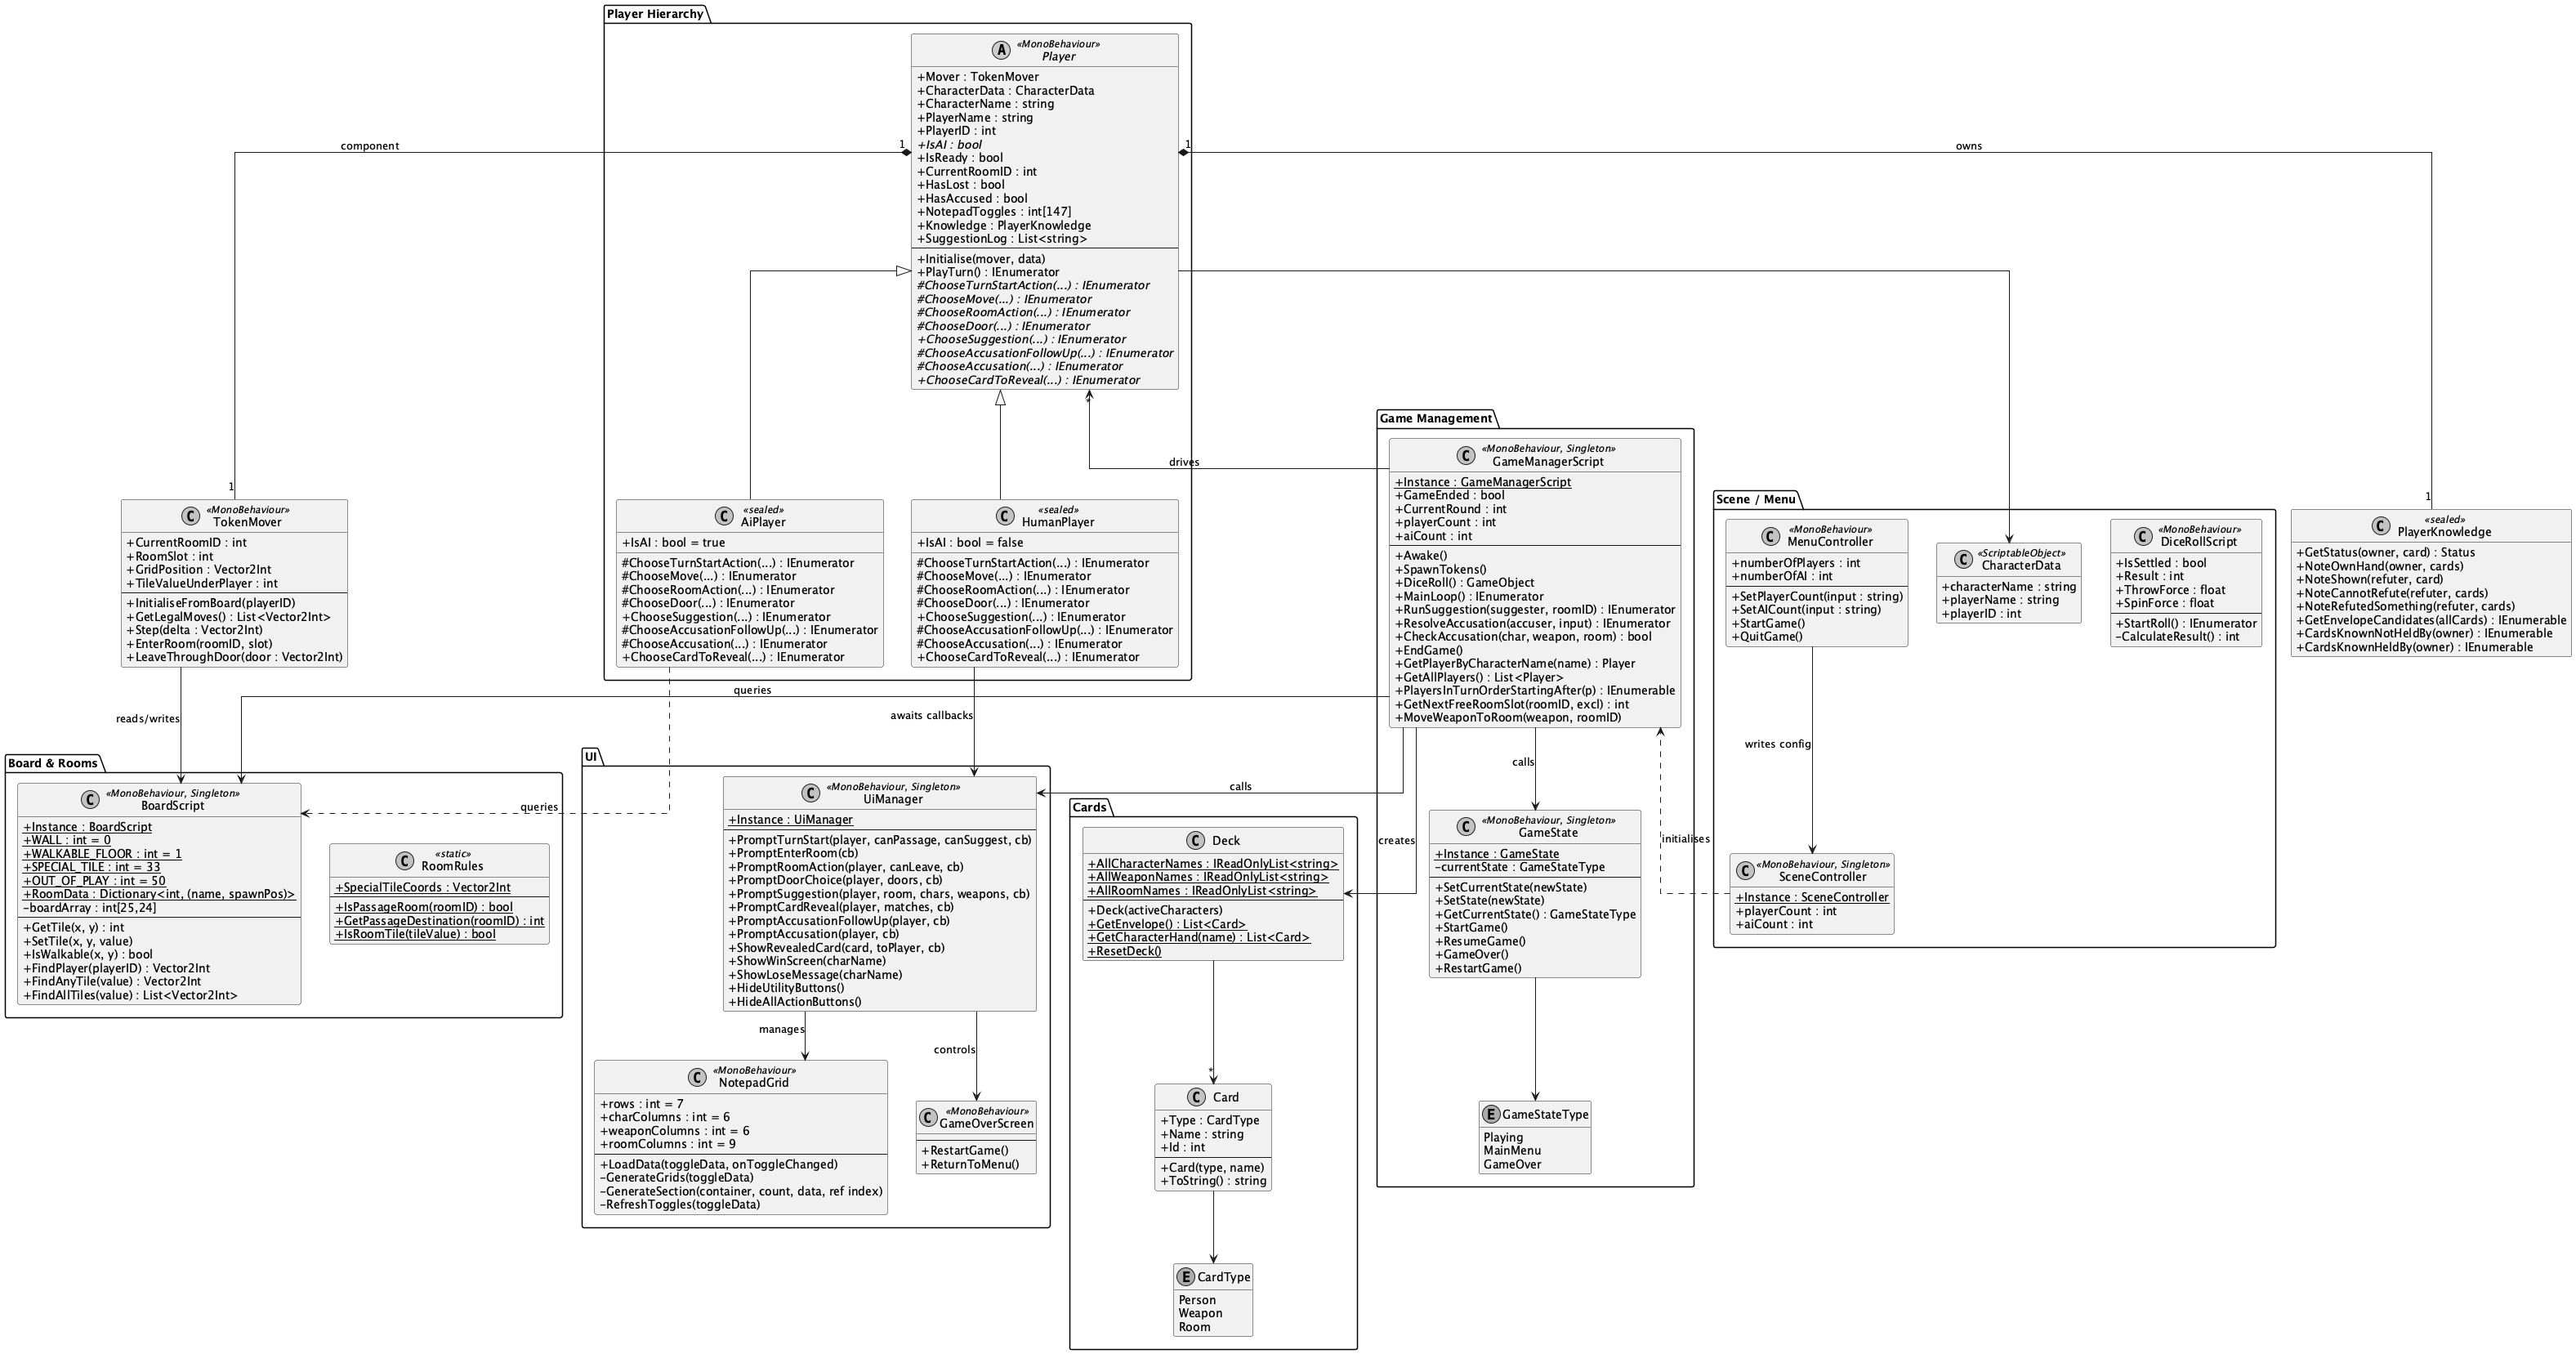
\includegraphics[width=\textwidth]{class_diagram.png}
\caption{Full class diagram for all sprints (see also Figure \ref{fig:class-diagram} in Process section)}
\label{fig:class-diagram-low}
\end{figure}

\subsection*{Player Class Hierarchy}

The central inheritance hierarchy separates game-logic sequencing from input method:

\begin{table}[H]
\centering
\footnotesize
\setlength{\tabcolsep}{3pt}
\begin{tabular}{|p{1.8cm}|p{2cm}|p{6cm}|}
\hline
\textbf{Class} & \textbf{Kind} & \textbf{Role} \\ \hline
\texttt{Player} & abstract Mono\-Be\-haviour & Owns all turn sequencing (\texttt{PlayTurn}), board-position delegation, knowledge tracking (\texttt{PlayerKnowledge}), and 147-cell notepad state. Declares abstract decision hook methods. \\ \hline
\texttt{HumanPlayer} & sealed : Player & Overrides every decision hook by calling \texttt{UiManager} and awaiting a callback via \texttt{WaitUntil}. \\ \hline
\texttt{AiPlayer} & sealed : Player & Overrides decision hooks: BFS-directed movement toward target room, knowledge-filtered suggestions, envelope-based accusation trigger. Comments describe further upgrade paths. \\ \hline
\end{tabular}
\end{table}

\subsection*{Key Public Decision Hook Signatures (\texttt{Player})}

\begin{table}[H]
\centering
\footnotesize
\setlength{\tabcolsep}{4pt}
\begin{tabular}{|p{5.2cm}|p{4.5cm}|}
\hline
\textbf{Method (abstract / public)} & \textbf{When called} \\ \hline
\texttt{ChooseTurnStart\-Action(\allowbreak canPassage, canSuggest, \allowbreak Action<TurnAction>)} & At turn start: roll / take passage / suggest-in-place \\ \hline
\texttt{ChooseMove(legal\-Moves, canEnterRoom, \allowbreak canUseSpecial, \allowbreak Action<Vector2Int,bool,\allowbreak bool>)} & Each movement step while walking \\ \hline
\texttt{ChooseDoor(doors, \allowbreak Action<Vector2Int>)} & When leaving a multi-door room \\ \hline
\texttt{ChooseSug\-gestion(roomID, \allowbreak chars, weapons, \allowbreak Action<Suggestion\-Input>)} & When the player must produce a suggestion \\ \hline
\texttt{ChooseAccusation\-FollowUp(\allowbreak Action<bool>)} & Immediately after suggestion resolves \\ \hline
\texttt{ChooseAccusation(\allowbreak roomID, Action<\allowbreak AccusationInput>)} & When \texttt{ChooseAccusationFollowUp} returned true \\ \hline
\texttt{ChooseCardToReveal(\allowbreak matches, Action<Card>)} & When refuting another player's suggestion \\ \hline
\texttt{ChooseRoomAction(\allowbreak canLeave, \allowbreak Action<RoomAction>)} & When in a room: stay and suggest in place, or leave through a door \\ \hline
\end{tabular}
\end{table}

\section{Key Class APIs}

\subsection*{\texttt{GameManagerScript} (Singleton)}

\begin{table}[H]
\centering
\footnotesize
\setlength{\tabcolsep}{4pt}
\begin{tabular}{|p{4.2cm}|p{5.5cm}|}
\hline
\textbf{Method} & \textbf{Description} \\ \hline
\texttt{CheckAccusation(\allowbreak character, weapon, \allowbreak room) : bool} & Checks three named cards against \texttt{Deck.\allowbreak GetEnvelope()} \\ \hline
\texttt{RunSuggestion(\allowbreak suggester, \allowbreak roomID) : \allowbreak IEnumerator} & Clockwise card-showing round; updates all players' \texttt{PlayerKnowledge}; shows revealed card to suggester via \texttt{UiManager.ShowRevealedCard} \\ \hline
\texttt{ResolveAccusation(\allowbreak accuser, \allowbreak Accusation\-Input) : \allowbreak IEnumerator} & Calls \texttt{CheckAccusation}; triggers \texttt{EndGame()} on win or sets \texttt{HasLost=true} on incorrect guess \\ \hline
\texttt{PlayersInTurnOrder\-StartingAfter(suggester) \allowbreak : IEnumerable\allowbreak <Player>} & Returns players clockwise from the suggester for card-showing \\ \hline
\texttt{GetNextFreeRoomSlot(\allowbreak roomID, excluding) \allowbreak : int} & Returns the next unoccupied visual slot in a room (1--6) \\ \hline
\texttt{MoveWeaponToRoom(\allowbreak weaponName, \allowbreak roomID)} & Repositions a weapon token to the specified room's spawn point \\ \hline
\texttt{DiceRoll() \allowbreak : GameObject} & Instantiates the physics dice and starts its roll coroutine \\ \hline
\texttt{EndGame()} & Sets \texttt{GameEnded=true}, destroys board/tokens, calls \texttt{GameState.GameOver()} \\ \hline
\end{tabular}
\end{table}

\subsection*{\texttt{BoardScript} (Singleton)}

\begin{table}[H]
\centering
\footnotesize
\setlength{\tabcolsep}{4pt}
\begin{tabular}{|p{4.2cm}|p{5.5cm}|}
\hline
\textbf{Member} & \textbf{Description} \\ \hline
\texttt{GetTile(x, y) : int} & Returns tile value; 0 for out-of-bounds \\ \hline
\texttt{SetTile(x, y, value)} & Writes a tile value; used by \texttt{TokenMover} to encode occupancy \\ \hline
\texttt{IsWalkable(x, y) \allowbreak : bool} & Returns true iff tile value is $\geq 1$ and $< 50$ (not wall, not player-start) \\ \hline
\texttt{FindPlayer(playerID) \allowbreak : Vector2Int} & Scans board for tile value == playerID; returns \texttt{(-1,-1)} if not found \\ \hline
\texttt{FindAllTiles(value) \allowbreak : List<Vector2Int>} & Returns all board positions with the given tile value (used for door sets) \\ \hline
\texttt{static RoomData : \allowbreak Dictionary<int,(string,\allowbreak Vector3)>} & Room ID $\to$ (name, world-space spawn position) \\ \hline
\texttt{const WALL=0, WALKABLE\-\_FLOOR=1, SPECIAL\-\_TILE=33, OCCUPIED=50} & Named tile-encoding constants \\ \hline
\end{tabular}
\end{table}

\subsection*{\texttt{TokenMover} (per-player MonoBehaviour)}

\begin{table}[H]
\centering
\footnotesize
\setlength{\tabcolsep}{4pt}
\begin{tabular}{|p{4.2cm}|p{5.5cm}|}
\hline
\textbf{Method} & \textbf{Description} \\ \hline
\texttt{InitialiseFromBoard(\allowbreak playerID)} & Locates the player's tile on \texttt{BoardScript}, sets grid position and world position \\ \hline
\texttt{GetLegalMoves() \allowbreak : List<Vector2Int>} & Returns orthogonal adjacent tiles that pass \texttt{BoardScript.IsWalkable} \\ \hline
\texttt{Step(Vector2Int delta)} & Moves one step: restores old tile value, encodes new tile with playerID, updates world position \\ \hline
\texttt{EnterRoom(\allowbreak roomID, slot)} & Moves token to the room's visual slot position; sets \texttt{CurrentRoomID} and \texttt{RoomSlot} \\ \hline
\texttt{LeaveThroughDoor(\allowbreak Vector2Int door)} & Exits room: places token on door tile, clears \texttt{CurrentRoomID}/\texttt{RoomSlot} \\ \hline
\end{tabular}
\end{table}

\subsection*{\texttt{PlayerKnowledge}}

\begin{table}[H]
\centering
\footnotesize
\setlength{\tabcolsep}{4pt}
\begin{tabular}{|p{4.2cm}|p{5.5cm}|}
\hline
\textbf{Method} & \textbf{Description} \\ \hline
\texttt{NoteOwnHand(\allowbreak owner, cards)} & Seeds the knowledge base with cards the player holds \\ \hline
\texttt{NoteShown(\allowbreak refuter, card)} & Records that \texttt{refuter} definitely holds \texttt{card} (suggester saw it) \\ \hline
\texttt{NoteCannotRefute(\allowbreak refuter, cards)} & Records that \texttt{refuter} holds none of \texttt{cards} (they passed) \\ \hline
\texttt{NoteRefutedSomething(\allowbreak refuter, cards)} & Records a disjunction: \texttt{refuter} holds at least one of \texttt{cards} (other observers) \\ \hline
\texttt{GetEnvelopeCandiates(\allowbreak allCards)} & Returns cards not definitively held by anyone---the set of possible envelope cards \\ \hline
\end{tabular}
\end{table}

\section{Object-Oriented Design Principles}

\subsection*{Single Responsibility}
Each class has one clearly bounded job:
\begin{itemize}
    \item \texttt{BoardScript} --- board state only (tile values, occupancy, walkability)
    \item \texttt{TokenMover} --- grid movement and room entry/exit only
    \item \texttt{Player} --- turn sequencing and knowledge tracking only; never touches the board directly
    \item \texttt{DiceRollScript} --- physics dice and face-detection only
    \item \texttt{UiManager} --- UI display and input collection only
    \item \texttt{Deck} / \texttt{Card} --- card data, dealing, and envelope management only
    \item \texttt{PlayerKnowledge} --- per-player card inference only
    \item \texttt{NotepadGrid} --- detective notebook toggle UI only
\end{itemize}

\subsection*{Inheritance and Polymorphism}
\texttt{Player} is an abstract MonoBehaviour that declares all turn-sequencing logic in concrete methods (\texttt{PlayTurn}, \texttt{DoMovementBudget}, \texttt{DoSuggestionThenAccusation}) and exposes abstract ``decision hook'' methods that the two subclasses override independently.
\begin{itemize}
    \item Template Method pattern: \texttt{Player.PlayTurn()} defines the skeleton of the turn; \texttt{HumanPlayer} and \texttt{AiPlayer} supply the input strategy by overriding each hook.
    \item Open/closed: adding a new player type (e.g.\ a network player) requires only a new subclass --- no changes to \texttt{GameManagerScript} or \texttt{Player.PlayTurn()}.
\end{itemize}

\subsection*{Singleton (Restricted to True Globals)}
\texttt{GameManagerScript}, \texttt{BoardScript}, \texttt{UiManager}, \texttt{GameState}, and \texttt{SceneController} use the Unity Singleton pattern because they represent unique global state any script may access. Per-player classes (\texttt{Player}, \texttt{TokenMover}, \texttt{DiceRollScript}) are instantiated per character.

\subsection*{Separation of Data and Presentation}
\texttt{Card} and \texttt{Deck} are pure C\# classes with no \texttt{MonoBehaviour} dependency. All visual representation is handled by \texttt{UiManager}. This keeps game logic testable independently of Unity's rendering pipeline.

\subsection*{Encapsulation}
Board state is private inside \texttt{BoardScript} --- all access is via \texttt{GetTile} / \texttt{SetTile} / \texttt{IsWalkable}. \texttt{TokenMover} writes back to the board via \texttt{SetTile}, so \texttt{BoardScript} is always the single source of truth for occupancy. \texttt{Deck}'s static dictionaries are private; access is only through \texttt{GetCharacterHand} and \texttt{GetEnvelope}.

\subsection*{Data-Driven Design}
All card names are loaded from \texttt{StreamingAssets/cards.json} at runtime via \texttt{JsonUtility}. Adding or renaming a character, weapon, or room requires only a JSON edit --- no code change, no recompile.

\subsection*{Callback-Driven UI Decoupling}
\texttt{UiManager} communicates results back to game logic via \texttt{System.Action} delegates; \texttt{Player} coroutines wait via \texttt{WaitUntil}. This means the turn coroutine has no knowledge of how the UI is built --- the same \texttt{Player.PlayTurn()} code drives both human and AI turns.

\section{Design vs.\ Implementation Deviations}

The table below records where the delivered codebase differs from the original design. Each deviation is documented transparently.

\begin{table}[H]
\centering
\footnotesize
\setlength{\tabcolsep}{4pt}
\begin{tabular}{|c|p{2.4cm}|p{2.8cm}|p{2.4cm}|p{2.8cm}|}
\hline
\textbf{\#} & \textbf{Designed} & \textbf{Delivered} & \textbf{Why} & \textbf{Where} \\ \hline
D1 & Standalone \texttt{Suggestion} & Inside \texttt{GameManager\-Script} & Late integration risk & \texttt{GameManager\-Script.cs} \\ \hline
D2 & Standalone \texttt{Accusation} & Inside \texttt{GameManager\-Script} & Same as D1 & \texttt{GameManager\-Script.cs} \\ \hline
D3 & Notebook-based AI deduction & BFS + knowledge-filtered & Core features in S4 & \texttt{AiPlayer.cs} \\ \hline
D4 & Full A* pathfinding & Legal-move navigation & Sprint 3 complexity & \texttt{TokenMover} \\ \hline
D5 & Single \texttt{TokenMovement\-Script} & Split into \texttt{Player} + subclasses & Separate concerns (S4) & 4 files \\ \hline
\end{tabular}
\end{table}

\section{Design Validation}

\subsection*{Sequence Diagrams}

The sequence diagrams are embedded in the sprint sections where the behaviour was first implemented:

\begin{itemize}
    \item \textbf{Player turn --- movement phase} (Figure \ref{fig:seq-movement}, Sprint 3): shows the interaction between \texttt{Player.PlayTurn()}, \texttt{TokenMover.GetLegalMoves()}, \texttt{HumanPlayer.ChooseMove()}, and \texttt{BoardScript}.
    \item \textbf{Suggestion resolution} (Figure \ref{fig:seq-suggestion}, Sprint 4): shows \texttt{GameManagerScript.RunSuggestion()} iterating players clockwise, calling \texttt{ChooseCardToReveal()} on the refuter, updating \texttt{PlayerKnowledge} on all observers, and calling \texttt{UiManager.ShowRevealedCard()} on the suggester.
\end{itemize}

\subsection*{Turn State Machine}

The turn state machine (Figure \ref{fig:state-turn}, Sprint 4) shows the states a player passes through within a single turn: \textit{Start} $\to$ \textit{ChooseAction} $\to$ \textit{Rolling/Moving/Passage} $\to$ \textit{InRoom} $\to$ \textit{Suggestion} $\to$ \textit{Accusation?} $\to$ \textit{End}.

% TODO: If the state machine diagram has been updated since the Sprint 4 image was generated
% (e.g. the ChooseTurnStartAction hook now also exposes a Suggest-in-place option),
% regenerate state_turn.puml and export a new state_turn.png to the overleaf/ folder.

\newpage

\chapter{Software Documentation}
\label{chap:software}

\section{Code Documentation Standard}

The codebase is implemented in C\# under Unity. All custom scripts adopt the C\#
XML documentation comment standard (triple-slash \texttt{///}) --- the idiomatic
equivalent of JavaDoc for the .NET ecosystem. This standard was chosen because
it is the native format consumed by Visual Studio, Visual Studio Code, and
JetBrains Rider for IntelliSense / hover tooltips, and because it can be
mechanically extracted into static HTML by tools such as DocFX or Sandcastle
without any further annotation work.

Every public type, public/internal member, and non-trivial private helper
carries at minimum a \texttt{<summary>} tag. Methods that take parameters or
return a meaningful value additionally carry \texttt{<param>} and
\texttt{<returns>} tags. Cross-references between related types use the
\texttt{<see cref="...">} tag so that IntelliSense renders clickable links.

\subsection*{Coverage}

\begin{table}[H]
\centering
\begin{tabular}{|l|r|}
\hline
\textbf{Metric} & \textbf{Count} \\ \hline
Custom C\# scripts in repository & 33 \\ \hline
Gameplay scripts (\texttt{Main Game/Scripts/}) & 22 \\ \hline
Menu / settings scripts (\texttt{Main Game/Menu/}) & 6 \\ \hline
Editor tooling (\texttt{Editor/}) & 1 \\ \hline
EditMode unit-test scripts (\texttt{Tests/EditMode/}) & 4 \\ \hline
Total \texttt{<summary>} doc tags & 209 \\ \hline
Total \texttt{<param>} / \texttt{<returns>} tags & 141 \\ \hline
\end{tabular}
\caption{XML documentation coverage across the custom codebase}
\end{table}

The XML documentation pass was committed in commit \texttt{b720a97}
(``Add XML documentation to all 29 custom C\# scripts''); the four test
scripts were documented inline as they were written. Unity-generated assets
(\texttt{TextMesh Pro}, \texttt{InputSystem\_Actions}, \texttt{OutlineEffect},
\texttt{UI Toolkit}, \texttt{Settings}) are excluded --- they are third-party
boilerplate, not authored team code.

\section{Documentation Conventions}

\subsection*{Class-level summaries}

Every class begins with a multi-line \texttt{<summary>} block describing its
single responsibility and any collaborators. For example, \texttt{PlayerKnowledge}
begins:

\begin{verbatim}
/// <summary>
/// Per-player inference about who holds which card. Populated by
/// GameManagerScript during suggestion resolution. Read by AiPlayer; in
/// a future PR, an "auto-fill notepad" toggle will project this into the
/// human's NotepadGrid.
///
/// Conceptually three tables of facts about the cards this player has
/// observed:
///   1. Definitely held by X       (saw X reveal it, or it's in own hand).
///   2. Definitely NOT held by X   (X passed on a suggestion containing
///                                  the card).
///   3. Held by exactly one of {X, cards}  (X refuted a suggestion but you
///                                          didn't see which card).
/// </summary>
public sealed class PlayerKnowledge { ... }
\end{verbatim}

\subsection*{Method-level documentation}

Public methods document their summary, parameters, and return value. The
following excerpt from \texttt{RoomRules.cs} is representative:

\begin{verbatim}
/// <summary>
/// Returns the room ID at the other end of the secret passage from
/// <paramref name="roomID"/>, or -1 if no passage exists.
/// </summary>
/// <param name="roomID">The room to travel from.</param>
/// <returns>Destination room ID, or -1.</returns>
public static int GetPassageDestination(int roomID) =>
    PassageMap.TryGetValue(roomID, out int d) ? d : -1;
\end{verbatim}

\subsection*{Enum and struct documentation}

Enum members and struct fields are documented individually so IntelliSense
explains each option at the call site. From \texttt{Player.cs}:

\begin{verbatim}
/// <summary>Actions available at the start of a turn (before or instead
/// of rolling).</summary>
public enum TurnAction
{
    /// <summary>Roll the dice and move.</summary>
    Roll,
    /// <summary>Use a secret passage to an adjacent room.</summary>
    Passage,
    /// <summary>Make a suggestion without rolling (only valid when already
    /// in a room).</summary>
    Suggest
}
\end{verbatim}

\subsection*{Inline comments}

Inline (\texttt{//}) comments are reserved for non-obvious algorithmic steps,
Unity-specific gotchas (e.g.\ Edit Mode vs.\ Play Mode coroutine constraints in
the test helpers), and rationale that would otherwise be lost. Self-explanatory
code is left uncommented to avoid noise.

\section{Documentation Tooling}

\begin{itemize}
    \item \textbf{IDE integration:} Visual Studio, VS Code (with the C\# Dev
    Kit), and JetBrains Rider all surface XML doc comments as hover tooltips
    and parameter hints. No separate build step is required --- every
    contributor sees the documentation while editing.
    \item \textbf{Static HTML generation:} the comments are compatible with
    DocFX (\texttt{docfx.exe}) and Sandcastle, which can produce a browsable
    HTML reference site directly from the source tree. This was not run for
    submission but the source is ready for it.
    \item \textbf{Compiler-checked references:} \texttt{<see cref="...">} tags
    are validated by the C\# compiler when the project is built with
    \texttt{/doc} enabled, catching stale references during refactors.
    \item \textbf{Project-level documentation:} architectural narrative,
    sprint records, and design diagrams live in the \texttt{report/} tree
    (Markdown and PlantUML sources, rendered into this report).
\end{itemize}

\section{Codebase Structure}

\subsection*{Repository layout}

\begin{table}[H]
\centering
\begin{tabular}{|p{6.2cm}|p{8cm}|}
\hline
\textbf{Path} & \textbf{Contents} \\ \hline
\texttt{README.md} & Setup guide: cloning, opening the project in Unity, Smart
Merge configuration, commit / PR workflow conventions \\ \hline
\texttt{clue/} & Unity project root (open this folder in Unity Hub) \\ \hline
\texttt{clue/Assets/Main Game/} & Game scene, prefabs, scripts \\ \hline
\texttt{clue/Assets/Main Game/Scripts/} & 22 gameplay scripts (board,
deck, player, AI, UI manager, etc.) \\ \hline
\texttt{clue/Assets/Main Game/Menu/} & 6 menu scripts (controller,
settings, stepper, modal, room plaque) \\ \hline
\texttt{clue/Assets/Editor/} & Editor-only tooling
(\texttt{ProjectFileGenerator.cs}) \\ \hline
\texttt{clue/Assets/Tests/EditMode/} & Sprint-aligned unit tests
(\texttt{Sprint1Tests.cs}\,--\,\texttt{Sprint4Tests.cs}) \\ \hline
\texttt{clue/Assets/StreamingAssets/} & \texttt{cards.json} --- runtime
data contract for the deck \\ \hline
\texttt{documentation/} & All design / planning / testing / meeting documentation
sources (Markdown + PlantUML) \\ \hline
\texttt{report/} & LaTeX source of this submission report \\ \hline
\end{tabular}
\caption{Repository layout and documentation locations}
\end{table}

\subsection*{Gameplay scripts at a glance}

Each script in \texttt{Main Game/Scripts/} owns a single responsibility,
documented in its class summary:

\begin{table}[H]
\centering
\resizebox{\textwidth}{!}{%
\begin{tabular}{|l|p{10cm}|}
\hline
\textbf{Script} & \textbf{Responsibility (from class \texttt{<summary>})} \\ \hline
\texttt{GameManagerScript.cs} & Central game controller: main turn loop, player
spawning, weapon placement, suggestion / accusation resolution \\ \hline
\texttt{BoardScript.cs} & 25$\times$24 tile grid; single source of truth for
walkability and occupancy \\ \hline
\texttt{DeckScript.cs} & Loads cards from \texttt{cards.json}, builds the
murder envelope, deals hands \\ \hline
\texttt{Player.cs} & Abstract base: turn state machine and decision hooks \\ \hline
\texttt{HumanPlayer.cs} & Player subclass: routes decisions through
\texttt{UiManager} \\ \hline
\texttt{AiPlayer.cs} & Player subclass: BFS-directed movement and
knowledge-filtered suggestions \\ \hline
\texttt{TokenMover.cs} & Grid movement, room entry / exit, world-space
positioning \\ \hline
\texttt{RoomRules.cs} & Static helper: secret-passage map and door-tile
detection \\ \hline
\texttt{DiceRollScript.cs} & Rigidbody dice; result decoded from face
orientation \\ \hline
\texttt{UiManager.cs} & Singleton entry point for every player-facing prompt \\ \hline
\texttt{NotepadUI.cs} & 147-cell detective-notebook toggle grid \\ \hline
\texttt{PlayerKnowledge.cs} & Per-player card inference (Held / NotHeld /
disjunctions) \\ \hline
\texttt{GameStateScript.cs} & Playing / MainMenu / GameOver state machine \\ \hline
\texttt{SceneController.cs} & Persists player and AI count between menu and
game scenes \\ \hline
\texttt{CharacterData.cs} & ScriptableObject: per-character static metadata \\ \hline
\texttt{GameOverScreen.cs} & End-of-game restart / return-to-menu UI \\ \hline
\texttt{CameraFollow.cs} & Smooth camera follow for the active player \\ \hline
\texttt{BoardThemer.cs} / \texttt{Theme Changer.cs} & Runtime board / menu
theme switching \\ \hline
\texttt{BakeData.cs} / \texttt{BakedNavData.cs} & Pre-computed navigation data
for AI BFS \\ \hline
\texttt{DiceDebugLogger.cs} & Editor-only diagnostic logger for dice physics \\ \hline
\end{tabular}%
}
\caption{Gameplay scripts and their documented responsibilities}
\end{table}

\section{Setup and Usage Guide}

The repository \texttt{README.md} is the canonical setup document. The key
steps it covers are:

\begin{enumerate}
    \item Clone the repository to a known location.
    \item Install the Unity version pinned in the project (Unity Hub will
    prompt if a different version is opened).
    \item In Unity Hub, click \textit{Add} $\to$ select the \texttt{clue}
    folder.
    \item Open \textit{Assets / Main Game / MenuScene} 
    press \textit{Play}.
\end{enumerate}

\noindent The README additionally documents the team's commit-message
expectations (testing notes, design rationale, collaboration evidence, risk
assessment, task attribution) and the branching strategy (feature branches per
sprint, merged via reviewed pull requests).

\newpage

\chapter{Project Overview}
\label{chap:project-overview}

\section{Team Members}

\begin{longtable}{llp{8cm}}
\toprule
\textbf{Name} & \textbf{GitHub Username} & \textbf{Role(s)} \\
\midrule
\endhead
Matt & Smelly21 & Frontend lead --- UI/GUI, board rendering, player HUD, detective notepad, menus \\
Ewan & KE41 & Game logic \& rules --- \texttt{GameManagerScript}, turn flow, suggestions, accusations, win conditions \\
Joe & Joseph-pb & Board \& movement --- board grid, rooms, doors, movement logic, secret passages; report and documentation lead \\
Ethan & BigRapturey123 & Board \& movement --- board grid, rooms, doors, movement edge cases, integration testing \\
Ben & 17bclarke & Card system --- Card/Deck classes, dealing, murder envelope; \texttt{DiceRollScript}; AI player \\
Edward & edward-baker05 & Data handling --- JSON schema design, \texttt{DeckScript} refactor, repo tooling (Git LFS, PR templates, Unity merge settings), \texttt{MenuController}, integration merges \\
\bottomrule
\end{longtable}

\section{About This Project}

\subsection{Project Description}

This report documents the development of a computer simulation of the classic board game Clue! (Cluedo) for the fictional client Watson Games. The system was developed in Unity (C\#) over four Agile sprint cycles between February and April.

The final deliverable is a desktop game for Mac/PC that supports multiple players (human or AI), featuring:
\begin{itemize}
    \item A faithful 25-row $\times$ 24-column tile representation of the Clue! board with all 9 rooms, corridors, doors, starting squares and secret passages
    \item Physics-based dice rolling (Rigidbody simulation with a fallback for degenerate results)
    \item Orthogonal token movement along corridors, bounded by the dice roll, with room entry detection
    \item A 21-card deck (6 characters, 6 weapons, 9 rooms) dealt from a 3-card murder envelope, with private per-player hand display
    \item Suggestion system: clockwise card-showing round with private card reveal via modal, and suggested token movement into the suggestion room
    \item Accusation evaluation against the murder envelope, with win condition and player elimination
    \item An AI player that takes full turns (roll, move, suggest, optionally accuse) without human input using BFS and basic knowledge tracking
    \item Per-player detective notepad (147-cell toggle grid)
    \item Game-over screen with restart and return-to-menu options
    \item Data-driven card names loaded from \texttt{cards.json} --- characters, weapons and rooms are configurable without recompiling
\end{itemize}

\section{How the Team Was Organised}

We did not formally designate a Scrum Master. Roles were assigned by area of responsibility at Meeting 3 (19/02/2026), with each team member owning one or two scripts per sprint. Matt took responsibility for all frontend/Unity rendering work. Ewan owned the core game logic and turn management. Joe and Ethan shared board and movement. Ben owned the card system, dice, and AI player. Edward owned data handling, JSON integration, and all repository tooling.

Code review was conducted via GitHub Pull Requests. Edward set up a PR template and a Unity compile-check workflow on PRs so that broken builds could not land on \texttt{master}. Each team member was responsible for documenting their own commits in the agreed schematic format.

\subsection{Technology Choices}
\begin{itemize}
    \item \textbf{Unity / C\#}: Agreed unanimously at Meeting 1. The whole team had little to no Unity experience and saw it as a valuable learning opportunity. Unity provides built-in 3D rendering, Rigidbody physics (used for the dice), and cross-platform Mac/PC builds.
    \item \textbf{Backend/frontend architecture}: Agreed at Meeting 1 --- backend outputs a game state; Matt's frontend consumes it. \texttt{GameManagerScript} is the single bridge; UI scripts never read board or deck state directly. This kept game logic testable independently of Unity's rendering pipeline.
    \item \textbf{Data-driven design}: All card names (characters, weapons, rooms) loaded from \texttt{StreamingAssets/cards.json} via \texttt{JsonUtility}. Agreed at Meeting 3, satisfying Watson Games' customisation requirement. Changing a character or room name requires only a JSON edit --- no recompile.
    \item \textbf{C\# XML doc comments}: Agreed at Meeting 3 as the documentation standard. IDE-surfaced hover tooltips; compatible with DocFX for HTML generation.
\end{itemize}

\subsection{Version Control}
We used \textbf{Git / GitHub} throughout. Branching strategy: feature branches per task $\rightarrow$ PR review $\rightarrow$ merge to \texttt{master}. Git LFS was configured in Sprint 2 for Unity binary files. Unity Smart Merge (\texttt{.gitattributes} for \texttt{.unity} and \texttt{.prefab}) was set up by Edward in Sprint 2 to prevent destructive scene-file merge conflicts.

\section{Sprint Summary}

\begin{longtable}{llp{5cm}p{4cm}}
\toprule
\textbf{Sprint} & \textbf{Dates} & \textbf{Key Deliverables} & \textbf{Prototype State} \\
\midrule
\endhead
Sprint 1 & 19 Feb -- 05 Mar & Planning, role assignments, Unity project setup; \texttt{Card}, \texttt{Deck}, \texttt{SceneController} classes; \texttt{cards.json} schema & Compiles and runs; no visual game yet \\
Sprint 2 & 05 -- 17 Mar & \texttt{BoardScript} (25$\times$24 tile grid), \texttt{GameManagerScript} singleton, \texttt{DiceRollScript} (Rigidbody), token spawning; repo tooling (Git LFS, PR templates, Unity merge settings) & Board visible; tokens spawn; dice rolls; no movement \\
Sprint 3 & 17 Mar -- 14 Apr & \texttt{TokenMovementScript} (corridor movement, room entry, occupancy), \texttt{UiManager} (suggestion/card reveal prompts), \texttt{NotepadGrid}, \texttt{HandManager}/\texttt{CardInteraction} & Playable board: move tokens, view hand, enter rooms; suggestion prompt appears \\
 Sprint 4 & 14 -- 30 Apr & \texttt{GameManagerScript.MainLoop()} full turn cycle; \texttt{RunSuggestion()} clockwise card-showing; accusation evaluation; AI player (BFS + Basic game state knowledge); \texttt{GameOverScreen}; system testing; documentation & Full playable game with documented limitations (KI-1 through KI-3) \\
\bottomrule
\end{longtable}

\section{Key Achievements}

\begin{itemize}
    \item \textbf{Board}: A 25$\times$24 tile grid (\texttt{BoardScript}) encodes all 9 rooms (tile values 2--11), corridors (value 1), walls (value 0), door squares and character starting squares. Room layout faithfully reproduces the standard Cluedo board. Evidence: \texttt{BoardScript.cs}, Section~\ref{sec:sprint2}, submission video.
    \item \textbf{Physics dice}: \texttt{DiceRollScript} uses a Unity Rigidbody simulation rather than \texttt{Random.Range}, giving the dice a visible roll animation. Face orientation is decoded by dot product against \texttt{Vector3.up}; a \texttt{Random.Range(1,7)} fallback handles any degenerate result. Risk R5 (dice giving zero results) never triggered in testing. Evidence: \texttt{DiceRollScript.cs}, Section~\ref{sec:sprint2}.
    \item \textbf{Movement}: Orthogonal token movement bounded by the dice roll value, with occupancy tracking (two tokens cannot share a corridor square), room-entry detection, and secret-passage support. Full A* pathfinding was deliberately descoped in favour of legal-move detection on the current roll --- documented as a design decision, not a defect. Evidence: \texttt{TokenMover.cs}, Section~\ref{sec:sprint3}.
    \item \textbf{Card system}: A 21-card deck (6 characters, 6 weapons, 9 rooms) loaded from \texttt{cards.json}. Three cards (one of each type) are selected as the murder envelope before dealing; remaining 18 are dealt round-robin. Each player's hand is displayed in a private UI visible only to that player. Evidence: \texttt{DeckScript.cs}, \texttt{HandManager.cs}, \texttt{cards.json}.
    \item \textbf{Suggestion and accusation}: End-to-end suggestion flow --- the suggesting player's character and weapon are named, the room is fixed as the current room, and the suggested character token is moved into the room. A clockwise card-showing round follows: each player in turn is prompted to reveal one matching card privately (via \texttt{UiManager.ShowRevealedCard}), ending when the first match is shown. Accusations are evaluated against \texttt{Deck.GetEnvelope()}: a correct accusation triggers the win screen; an incorrect one eliminates the player from future turns while keeping their hand available for responses. Evidence: \texttt{GameManagerScript.cs}, \texttt{UiManager.cs}, Section~\ref{sec:sprint4}.
    \item \textbf{AI player}: \texttt{AiPlayer} takes full turns without human input --- rolls dice, selects a good legal move (BFS-directed toward envelope-candidate rooms), enters rooms and makes a suggestion from the character and weapon cards not yet eliminated from its knowledge base, and accuses when envelope candidates narrow to exactly 3. Each turn completes in under 5 seconds. Evidence: \texttt{AiPlayer.cs}, Section~\ref{sec:sprint4}.
    \item \textbf{Detective notepad}: A 147-cell toggle grid (\texttt{NotepadGrid} / \texttt{NotepadUI.cs}) is available per human player. It persists across turns and allows players to manually track which cards have been shown. Evidence: \texttt{NotepadUI.cs}, Section~\ref{sec:sprint3}.
    \item \textbf{Process and engineering}: Nine documented team meetings with agreed actions and completion tracking; four sprint cycles each with retrospectives; PR-driven workflow with Unity compile checks on every PR preventing broken builds from landing on \texttt{master}; Git LFS and UnityYAMLMerge preventing destructive scene-file conflicts after Sprint 2. Evidence: Section~\ref{sect:meeting}, Table~\ref{tab:risk_register} (Sprint~2 row), GitHub PR history.
\end{itemize}

\section{Outstanding Issues and Known Bugs}

\begin{longtable}{lp{4cm}p{4cm}p{4cm}}
\toprule
\textbf{Issue} & \textbf{Description} & \textbf{Why it exists} & \textbf{What we'd do with more time} \\
\midrule
\endhead
KI-1 & AI player makes basic suggestion decisions only --- it eliminates cards from its notepad based on what it has observed, but does not use probability to remove inferred cards & Deeper deduction logic was scoped down in Sprint 4 due to time pressure; the \texttt{PlayerKnowledge} scaffold is in place & Layer probability-elimination deduction on top of the base using \texttt{PlayerKnowledge.GetEnvelopeCandidates()} --- the architecture already supports this \\
KI-2 & Suggestion / Accusation logic lives inside \texttt{GameManagerScript.cs} and \texttt{UiManager.cs} rather than as standalone classes & Late integration timeline in Sprint 4 did not allow a clean refactor without risking the deadline; accepted as a deliberate trade-off & Extract \texttt{Suggestion} and \texttt{Accusation} into their own classes; add focused unit tests for each \\
KI-3 & Test S4.7 (F4.5): suggested character and weapon tokens do not fully move to the suggestion room. \texttt{RunSuggestion()} calls \texttt{target.Mover.EnterRoom()} only when \texttt{GetPlayerByCharacterName()} returns non-null and the target is not the suggester; \texttt{MoveWeaponToRoom()} is called unconditionally. This means that tokens that aren't spawned won't be placed in the room if suggested. & Root cause is simply the tokens not being marked as active if they aren't involved in the game; a fix was not attempted due to time constraints & Trace the exact failing path (null character lookup, suggester = target, or positioning error in \texttt{EnterRoom()}/\texttt{MoveWeaponToRoom()}); add a unit test asserting both token positions after \texttt{RunSuggestion()} \\
\bottomrule
\end{longtable}


\section{What Went Well}

\begin{itemize}
    \item \textbf{Repository tooling prevented merge disasters}: Setting up Git LFS, \texttt{.gitattributes} for Unity Smart Merge, and PR templates at the start of Sprint 2 (Meeting 4 actions, completed 6--7 March by Ethan and Edward) eliminated Unity scene and prefab merge conflicts for the rest of the project. Risk R2 materialised in Sprint 2 and was immediately contained; it did not recur. Without this tooling, late-sprint parallel feature work would have been extremely fragile.
    \item \textbf{Parallel development by area kept work non-blocking}: Assigning ownership of one or two scripts per person per sprint (agreed at Meeting 3) meant team members rarely blocked each other. The card system (Ben), board rendering (Matt), game manager (Ewan), and movement (Joe, Ethan) all progressed in parallel across Sprints 2--3 with minimal dependency conflicts. Evidence: Table~\ref{tab:gantt_tasks} (owners column).
    \item \textbf{Architecture decisions made early paid off throughout}: The backend/frontend separation (Meeting 1), the \texttt{GameManagerScript} singleton as the single bridge (Meeting 5), and the data-driven \texttt{cards.json} approach (Meeting 3) were all agreed before coding began. These decisions kept each area independently developable and meant Watson Games' customisation requirement could be satisfied in the future without any rework.
    \item \textbf{End-to-end delivery of Sprint 4 critical path}: Every critical-path objective for Sprint 4 shipped --- full turn cycle, clockwise suggestion resolution, accusation evaluation, AI player, and game-over screen. The late-sprint integration push (Edward's large branch merge on 18 April, followed by collaborative work from Ewan, Edward, and Ethan on suggestion logic) consolidated all major feature branches without losing work.
    \item \textbf{Honest documentation of limitations}: Rather than silently leaving known bugs undocumented, the team logged known issues (KI-1 through KI-3) explicitly in Section~\ref{sec:sprint4} and Section~\ref{sec:sprint4-known-issues} of this report.
    \item \textbf{Risk R5 and R6 never materialised}: The physics dice fallback (R5) and the random-AI fallback approach (R6) were both planned defensively from Sprint 1 and neither became a problem. The dice never returned an invalid result in testing; the AI approach was scoped fairly from the start.
\end{itemize}

\section{What Didn't Go Well / Lessons Learned}

\begin{itemize}
    \item \textbf{Easter break was not budgeted into the plan}: The 3.5-week Easter pause (20 March -- 14 April) was completely foreseeable but not reflected in the Gantt chart or sprint dates. The plan assumed continuous progress through Sprint 3. In reality, Sprint 3 work was compressed into the period 15--24 April, overlapping heavily with Sprint 4 and creating significant time pressure. \textit{Lesson: cost all known vacation windows into the plan from day one.}
    \item \textbf{Sprint 2 lost approximately one week to unplanned repository tooling}: Git LFS setup, \texttt{.gitignore} fixes, PR templates, Unity merge settings and the compile-check workflow were all necessary --- but should have been done in Sprint 1 before any feature work began. The plan did not budget this time, so Sprint 2 feature tasks arrived late. \textit{Lesson: front-load all toolchain work on day one of Sprint 1, before feature branches open.}
    \item \textbf{TokenMovement was harder than estimated and slipped}: The planned end date was 15 April; significant movement fixes landed on 17--18 April (Ethan's ``fixed movement'' and Edward's large merge). Legal-move detection on the irregular Cluedo board required substantially more edge-case handling than anticipated, and the task blocked development for everything downstream. \textit{Lesson: for the longest single task, add an explicit buffer and consider stubbing the interface earlier so other work can proceed.}
    \item \textbf{Late integration push created architectural debt}: Because the game loop, suggestion, accusation and AI player all converged in the final 10 days, the Suggestion and Accusation classes could not be extracted cleanly --- they were merged into \texttt{GameManagerScript} and \texttt{UiManager} under time pressure (KI-2). \textit{Lesson: stub the end-to-end game loop in Sprint 1, even if every action just logs to the console. Building outwards from a working skeleton would have surfaced integration problems much earlier.}
    \item \textbf{Documentation was partly reconstructed rather than maintained in real time}: Several sprint docs were filled in retrospectively during the Sprint 4 documentation push rather than being written as each sprint ran. This cost effort near the deadline and made it harder to verify exact timelines. \textit{Lesson: designate one person per sprint to maintain the sprint doc live, not retroactively.}
    \item \textbf{Two of the final five meetings were held without Matt}: Meetings 8 and 9 were attended by Ben, Edward, Ethan, Ewan and Joe only. Some Sprint 4 UI integration decisions were made without Matt's direct input and required follow-up via async communication, adding friction at a critical time. \textit{Lesson: agree a minimum-attendance rule early; if a member cannot attend, ensure decisions are communicated to them within 24 hours with an explicit confirmation required.}
    \item \textbf{Sprint~4 system tests were not fully executed before submission}: The system test table (S4.1--S4.12, Section~\ref{sec:sprint4}) has complete test cases and expected outputs, but Actual Result and Pass/Fail columns could not be filled in before the deadline. This is the most significant gap against the 9--10 testing band, which requires full documentation including pass/fail verdicts. The test cases are requirements-linked (F4.x / NF4.x), which partially satisfies the 7--8 band criterion.
    \item \textbf{AI player does not reach full deduction sophistication}: The \texttt{AiPlayer} uses BFS-directed navigation toward envelope-candidate rooms and filters suggestions against its \texttt{PlayerKnowledge} base, but does not perform full card-elimination deduction (D3, KI-1). \\ 
    \item \textbf{Watson Games' customisation requirement only partially met}: The brief explicitly identifies customisation as a selling point. The team delivered four selectable board themes (Section~\ref{chap:appendix}), but player names are not user-configurable. Weapon and character art packs loadable from data files were identified as future work but not delivered, but this only requires creating the assets and giving a menu on the front end. On the back end, the logic for this exists.
    \item \textbf{No animated visual appearance}: The physics-based dice provides some animation, but character tokens do not animate on movement. 
\end{itemize}

\section{What We Would Do Differently}

\begin{itemize}
    \item \textbf{Stub the end-to-end game loop in Sprint 1.} Even if every action is a \texttt{Debug.Log}, a working turn cycle (roll $\rightarrow$ move $\rightarrow$ suggest $\rightarrow$ accuse $\rightarrow$ win check) from the very beginning would have given every other system a defined interface to plug into. Instead, token movement, suggestion and accusation were all urgent in Sprint 4 precisely because the loop did not exist earlier.
    \item \textbf{Treat the Easter break as a hard Sprint 3 deadline, not a mid-sprint pause.} Sprint 3 should have closed its deliverables before 20 March. Planning the sprint to finish \textit{before} Easter would have preserved Sprint 4 as a genuine testing and integration buffer rather than a compressed feature sprint.
    \item \textbf{Set up all repository tooling on day one of Sprint 1.} Git LFS, \texttt{.gitattributes}, Unity Smart Merge, PR templates and the compile-check workflow should all be done before the first feature branch opens. Toolchain failures early in a sprint cascade into feature delays.
    \item \textbf{Allocate one person per sprint to maintain documentation alongside development.} A rotating ``sprint scribe'' role --- someone responsible for keeping the sprint doc current throughout the sprint rather than at the end --- would have prevented the retroactive reconstruction near the deadline.
    \item \textbf{Define a minimum viable AI contract early, then expand.} The random-decision AI was the right minimum; the architecture (\texttt{PlayerKnowledge}, abstract decision hooks on \texttt{Player}) was well designed for layering on deduction. However, this design should have been locked in Sprint 1 and expanded incrementally, rather than being finalised under Sprint 4 time pressure with deduction left unimplemented.
\end{itemize}

\section{Ideas for Further Development}

\begin{itemize}
    \item A smarter AI player using card-elimination deduction logic (the \texttt{PlayerKnowledge} scaffold is already in place --- \texttt{GetEnvelopeCandidates()} is implemented and wired into the AI)
    \item Animated token movement along the path (rather than step-by-step per key press)
    \item Online/networked multiplayer support (the abstract \texttt{Player} base class with decision hooks would accommodate a \texttt{NetworkPlayer} subclass without changes to \texttt{GameManagerScript})
    \item Custom board, character and weapon packs loaded from Watson Games data files (foundation already in place via \texttt{cards.json})
    \item Mobile port (Unity's cross-platform build targets make this achievable; touch input would need to replace keyboard movement)
\end{itemize}

\section{Peer Assessment}
\label{sec:peer-assessment}

\begin{quote}
\textbf{120 points total to distribute} (6 members $\times$ 20 points). Marks must be agreed by every team member. Justifications reference concrete contributions --- specific scripts, docs, or sprint outcomes --- not personality or generic effort claims.

Effort allocation from Table~\ref{tab:effort}: Edward 52 h, Ethan 49 h, Ewan 45 h, Joe 45 h, Ben 40 h, Matt 40 h (total $\approx$ 270 h). The peer marks below represent the fact that everyone equally did their parts.
\end{quote}

\begin{longtable}{llp{9cm}}
\toprule
\textbf{Team Member} & \textbf{Peer Mark} & \textbf{Justification} \\
\midrule
\endhead
Matt & 20 & Unity project setup (clue), BoardScript scene work, UiManager (PromptSuggestion / PromptCardReveal / ShowRevealedCard), NotepadGrid UI, CardGenerator/HandManager, GameOverScreen, main menu. Significant scene/prefab contributions that do not appear as script commits. \\
Ewan & 20 & GameManagerScript (MainLoop, RunSuggestion, ResolveAccusation, EndGame), GameStateScript, turn cycle design, menu scene transitions, coordinated Sprint 4 critical-path delivery. \\
Joe & 20 & TokenMovementScript (corridor movement, room entry, DragIntoRoom integration), branching/workflow documentation, board representation planning, Sprint documentation and report lead across all sprints. \\
Ethan & 20 & Git LFS and master/development branch cleanup (Sprint 2), TokenMovementScript movement edge cases and fixes (17--18 April integration), suggestion loop bug fix (``fixed suggestion to loop over everyone''), room entry integration testing. \\
Ben & 20 & Card / Deck classes and cards.json, DiceRollScript (Rigidbody physics + fallback), HandManager / CardInteraction / CardGenerator, AI player decision methods (move selection, suggestion generation, accusation trigger). \\
Edward & 20 & cards.json schema design, DeckScript refactor, SceneController, MenuController, PR/issue templates, Unity compile-check workflow, Git LFS setup, Unity merge settings, ``Large merge of all major branches'' (18 Apr), guessing/suggestion logic contribution, ongoing integration and documentation, refactored TokenMovementScript into separate classes, helped others when they fell behind. \\
\bottomrule
\end{longtable}

\noindent All team members agree to the above distribution:
\begin{itemize}
    \item Matt: MW
    \item Ewan: EM
    \item Joe: JB
    \item Ethan: EA
    \item Ben: BC
    \item Edward: EB
\end{itemize}

\section{Weekly Progress Log}

\begin{longtable}{llp{10cm}}
\toprule
\textbf{Week} & \textbf{Dates} & \textbf{Progress} \\
\midrule
\endhead
Week 1 & 26 Jan -- 01 Feb & Meeting 1 (29/01): project briefing reviewed; Unity/C\# agreed; frontend/backend architecture agreed; Matt designated frontend lead. Edward: Unity project created and set up.  \\
Week 2, 3 & 02 -- 15 Feb & Meeting 2 (02/02): Unity spike confirmed working on all machines; class diagram approach agreed; risk register initiated; commit schematic format agreed. Basic game setup commits. Risk register drafted (Joe, Edward). \\
Week 4 & 16 -- 22 Feb & Meeting 3 (19/02): role assignments finalised; sprint plan agreed; XML doc comments standard set; privacy model (Option B --- private modal) agreed; data-driven JSON approach confirmed. Joe: report/ skeleton committed; meeting notes written up. \\
Week 5 & 23 Feb -- 01 Mar & Sprint 1 work underway: Ben implementing Card/Deck classes; Edward designing \texttt{cards.json} schema and SceneController; Joe and Ethan on board/movement planning. \\
Week 6 & 02 -- 08 Mar & Meeting 4 (05/03): Sprint 1 closed; all objectives met. Sprint 2 plan agreed. Ethan: Git LFS and branch cleanup (06/03). Edward: PR templates, Unity merge settings, compile-check workflow (07/03). Matt: initial Unity project pushed (07/03). \\
Week 7 & 09 -- 15 Mar & Meeting 5 (10/03): backend/frontend boundary clarified; Matt explained Unity to the team; Deck refactor agreed. Edward: Deck refactor, GameManager scaffold, token spawning started (11--17 Mar). Ewan: GameManagerScript. Ben: DiceRollScript. \\
Week 8 & 16 -- 22 Mar & Meeting 6 (17/03): Sprint 2 review; GameState singleton agreed; Joe and Ethan assigned to TokenMovementScript; SceneController DontDestroyOnLoad agreed. Sprint 2 closed. Ewan: GameStateScript. Joe/Ethan: TokenMovementScript begun. \\
Week 9, 10, 11 & 23 -- 12 Apr & [Easter break --- no commits] \\
Week 12 & 13 -- 19 Apr & TokenMovementScript: corridor movement and occupancy tracking working; UiManager scaffolded by Matt; RoomScript door mapping started by Ben. Meeting 8 (14/04): Sprint 3 closed; suggestion resolution identified as top Sprint 4 priority; known issue KI-1 logged for documentation. UiManager completed (Matt). NotepadGrid working (Matt). Room entry detection done (Joe/Ethan). CardInteraction and GameOverScreen committed. Edward: large merge of all major branches (18 Apr). \\
Week 13 & 20 -- 26 Apr & Meeting 9 (20/04): suggestion resolution working end-to-end; accusation logic complete; TokenMovementScript refactored to allow for easier AI implementation; AI player taking full turns; GameOverScreen wired. Ethan: suggestion loop fix. Ben: AI suggestion generation. Documentation push begun (Joe lead). \\
Week 14 & 27 -- 01 May & Testing, documentation completion (sprint docs, group report, system testing), peer assessment agreement, video recording (Ethan), submission ZIP preparation and upload to Canvas. \\
\bottomrule
\end{longtable}


\appendix
\chapter{Appendix: AI Use Declaration}
\label{chap:appendix}

\section*{Generative AI --- Board Theme Assets}

Three of the four selectable board themes in the game use texture images generated with \textbf{Gemini} (Google DeepMind), a generative AI image model. The affected themes and their corresponding asset files are:

\begin{itemize}
    \item \textbf{Futuristic} --- \texttt{Gemini\_Generated\_Image\_8hp7e18hp7e18hp7.png}
    \item \textbf{Space Ship} --- \texttt{Gemini\_Generated\_Image\_f7l6o8f7l6o8f7l6.png}
    \item \textbf{Steampunk} --- \texttt{f554b52e-cbd9-4b91-aa0f-081b42186313.jpg}
\end{itemize}

These images are applied to the board 3D object at runtime via \texttt{BoardThemer.cs}, with the player's selection persisted through Unity's \texttt{PlayerPrefs} system (\texttt{"BoardTheme"} key) and exposed to the player via the in-game settings panel (\texttt{SettingsController.cs}). The default \textbf{Standard} theme uses the original Cluedo board image (\texttt{cluedoboard.jpg}) and is not AI-generated.

No generative AI was used for any written content, diagrams, code, or analytical work in this report or the accompanying software.


\end{document}
